% #############################################################################
% This is the MAIN DOCUMENT of the Thesis MSc TEMPLATE.
% The content for the Thesis MSc is to be written in separate documents
% located in the folder ./Chapters
%         Aknowledgments.tex
%         Abstract.tex
%         KeyWords.tex
%         Resumo.tex
%         PalavrasChave.tex
%         Acronyms.tex
%         Front_Cover.tex
%         Chapter_1.tex ....Chapter_2 .....
%         ApendixA.tex ... ApendixB.tex...
% -----------------------------------------------------------------------------
% The class "istulthesis" is based on the standard LaTeX 'report' class.
% It can be used for Instituto Superior Tecnico thesis, as it follows the 
% regulations published by the Scientific Council of IST.
% The class defines the document style. 
% IST requires the thesis to be written in Arial or similar. 
% Two arguments in '\documentclass' allow you to define the thesis font: 
% 'Helvetica' and 'AvantGarde', which transforms 
% the default LaTeX font into Helvetica or AvantGarde, respectively.
% #############################################################################
% The document is automatically set for english or portuguese by just selecting
% the MAIN LANGUAGE in file 'Thesis-MSc-Preamble_commands.tex' 
% #############################################################################
% Thesis-MSc
% Version 4.1, January 2023
% BY: Prof. Rui Santos Cruz, rui.s.cruz@tecnico.ulisboa.pt
% #############################################################################
% !TEX root = ./main.tex
% -----------------------------------------------------------------------------
%
%\documentclass[defaultstyle,10pt,Helvetica,oneside]{istulthesis}
\documentclass[defaultstyle,10pt,Helvetica,twoside,openright]{istulthesis}
%
% -----------------------------------------------------------------------------
% The Preamble document contains all the necessary Packages for typesetting
% Modify it to suit your needs
% -----------------------------------------------------------------------------
% #############################################################################
% Preamble for Thesis-MSc in English or Portuguese
% Required Packages and commands
% --> Please Choose the MAIN LANGUAGE for the Thesis in package BABEL (below)
% !TEX root = ./main.tex
% #############################################################################
% Thesis-MSc
% Version 4.1, January 2023
% BY: Prof. Rui Santos Cruz, rui.s.cruz@tecnico.ulisboa.pt
% #############################################################################
%
% -----------------------------------------------------------------------------
% PACKAGES ucs, utf8x, babel, iflang:
% -----------------------------------------------------------------------------
% The 'ucs' package provides support for using UTF-8 in LaTeX documents. 
% However in most situations it is not required.
\usepackage{ucs}
% The 'utf8x' package contains support for using UTF-8 as input encoding. 
\usepackage[utf8x]{inputenc}
% The 'babel' package may correct some hyphenation issues of LaTeX. 
% Select your MAIN LANGUAGE for the Thesis with the 'main=' option.
\usepackage[main=english,portuguese]{babel}
% The 'iflang' package is used to help determine the language being used. 
\usepackage{iflang}

% -----------------------------------------------------------------------------
% PACKAGE scrbase:
% -----------------------------------------------------------------------------
% The 'scrbase' package is used to help redefining document structure.
\usepackage{scrbase}
% -----------------------------------------------------------------------------
% PACKAGE mathtools, amsmath, amsthm, amssymb, amsfonts, nicefrac:
% -----------------------------------------------------------------------------
% These packages are typically required. 
% Among many other things they add the possibility to put symbols in bold
% by using \boldsymbol (not \mathbf); defines additional fonts and symbols;
% adds the \eqref command for citing equations.
\usepackage{mathtools, amsmath, amsthm, amssymb, amsfonts}
\usepackage{nicefrac}
%
% -----------------------------------------------------------------------------
% PACKAGE tikz:
% -----------------------------------------------------------------------------
% Tikz  for creating graphics programmatically.
\usepackage{tikz}
\usetikzlibrary{shapes.geometric, arrows, positioning}
% -----------------------------------------------------------------------------
% PACKAGES array, booktabs, multirow, colortbl, spreadtab:
% -----------------------------------------------------------------------------
% These packages are most usefull for advanced tables. 
% 'multirow' allows to join rows throuhg the command \multirow which works
% similarly with the command \multicolumn.
% The 'colortbl' package allows to color the table (foreground and background)
% The package 'booktabs' provide some additional commands to enhance
% the quality of tables
% The 'longtable' package is only required when tables extend beyond the length
% of one page, which typically does not happen and should be avoided
\usepackage{array}
\usepackage{booktabs}
\usepackage{multirow}
\usepackage{colortbl}
\usepackage{spreadtab}
\usepackage{longtable}
\usepackage{pdflscape}
\usepackage{float}
%
% -----------------------------------------------------------------------------
% PACKAGES graphicx, subfigure:
% -----------------------------------------------------------------------------
% The package 'graphicx' supports formats PNG and JPG.
% Package 'subfigure' allows to place figures within figures with own caption. 
% For each of the subfigures use the command \subfigure.
\usepackage{graphicx}
\usepackage[hang,small,bf,tight]{subfigure}
%
% -----------------------------------------------------------------------------
% PACKAGE caption:
% -----------------------------------------------------------------------------
% The 'caption' package offers customization of captions in floating 
% environments such figure and table
% \usepackage[hang,small,bf]{caption}
\usepackage[format=hang,labelfont=bf,font=small]{caption} 
% the following customization adds vertical space between caption and the table
\captionsetup[table]{skip=10pt}
%
% -----------------------------------------------------------------------------
% PACKAGE algorithmic, algorithm, algorithm2e:
% -----------------------------------------------------------------------------
% These packages are required if you need to describe an algorithm.
% The preference is for using 'algorithm2e'
%\usepackage{algorithmic}
%\usepackage[chapter]{algorithm}
\usepackage[ruled,vlined,algochapter,norelsize,\languagename]{algorithm2e}
%
% -----------------------------------------------------------------------------
% PACKAGE listings
% -----------------------------------------------------------------------------
% These packages are required if you need to list code snippets.
\usepackage{listings}
% Nicely syntax highlighted m-code in LaTeX documents with stylefile mcode.sty
% http://www.mathworks.com/matlabcentral/fileexchange/8015-m-code-latex-package
\usepackage[numbered]{mcode}
%
% -----------------------------------------------------------------------------
% Re-define listings captions and titles based on language.
\newcaptionname{portuguese}{\lstlistingname}{Listagem} % Listings CAPTIONS
\newcaptionname{portuguese}{\lstlistlistingname}{Listagens} % LIST of LISTINGS
%
% -----------------------------------------------------------------------------
% PACKAGE csquotes
% -----------------------------------------------------------------------------
% Quotation helper package
\usepackage{csquotes}
%
% -----------------------------------------------------------------------------
% PACKAGE todonotes
% -----------------------------------------------------------------------------
% Create TODO Notes in text
% The notes can be made invisible by just using the 'disable' option:
\usepackage[textwidth=2cm, textsize=small]{todonotes}
%\usepackage[textwidth=2cm, textsize=small, disable]{todonotes}
\setlength{\marginparwidth}{2cm}
%
% -----------------------------------------------------------------------------
% PACKAGE changes
% -----------------------------------------------------------------------------
% Track changes in document (changes in pdf preview).
%% Use "final" option to make all tracking markups invisible.
%\usepackage[authormarkup=superscript,authormarkuptext=id,markup=underlined,ulem={ULforem,normalbf},final]{changes}
\usepackage[authormarkup=superscript,authormarkuptext=id,markup=underlined,ulem={ULforem,normalbf}]{changes}
% commands:
% \added[id=xx]{text}
% \deleted[id=xx]{text}
% \replaced[id=xx]{deleted text}{added text}
% -----------------------------------------------------------------------------
% PACKAGES xcolor, color
% -----------------------------------------------------------------------------
% These packages are required for list code snippets.
\usepackage{xcolor}
\usepackage{color}
% The following special color definitions are used in the IST Thesis
\definecolor{forestgreen}{RGB}{34,139,34}
\definecolor{orangered}{RGB}{239,134,64}
\definecolor{lightred}{rgb}{1,0.4,0.5}
\definecolor{orange}{rgb}{1,0.45,0.13}	
\definecolor{darkblue}{rgb}{0.0,0.0,0.6}
\definecolor{lightblue}{rgb}{0.1,0.57,0.7}
\definecolor{gray}{rgb}{0.4,0.4,0.4}
\definecolor{lightgray}{rgb}{0.95, 0.95, 0.95}
\definecolor{darkgray}{rgb}{0.4, 0.4, 0.4}
\definecolor{editorGray}{rgb}{0.95, 0.95, 0.95}
\definecolor{editorOcher}{rgb}{1, 0.5, 0} % #FF7F00 -> rgb(239, 169, 0)
\definecolor{chaptergrey}{rgb}{0.6,0.6,0.6}
\definecolor{editorGreen}{rgb}{0, 0.5, 0} % #007C00 -> rgb(0, 124, 0)
\definecolor{olive}{rgb}{0.17,0.59,0.20}
\definecolor{brown}{rgb}{0.69,0.31,0.31}
\definecolor{purple}{rgb}{0.38,0.18,0.81}
%
% -----------------------------------------------------------------------------
% PACKAGE setspace:
% ----------------------------------------------------------------------------
% Provides support for setting the spacing between lines in a document. 
% Package options include single spacing, one half spacing, and double spacing. 
% Alternatively the spacing can be changed as required with:
% \singlespacing, \onehalfspacing, and \doublespacing commands
\usepackage{setspace}
%
% -----------------------------------------------------------------------------
% PACKAGE paralist
% -----------------------------------------------------------------------------
% This package provides the 'inparaenum' environment for inline lists
\usepackage{paralist}
% usage:
% \begin{inparaenum}[(a)]
% \item bla
% \item bla, bla
% \end{inparaenum}
% -----------------------------------------------------------------------------
% PACKAGE cite:
% -----------------------------------------------------------------------------
% The 'cite' package will result in citation numbers being automatically
% sorted and properly "ranged". i.e.,
% [1], [2], [5]--[7], [9]
\usepackage{cite}
%
% -----------------------------------------------------------------------------
% PACKAGE acronym:
% -----------------------------------------------------------------------------
% The package 'acronym' garantees that all acronyms definitions are 
% given at the first usage. 
% IMPORTANT: do not use acronyms in titles/captions; otherwise the definition 
% will appear on the table of contents.
\usepackage[printonlyused]{acronym}
%
% -----------------------------------------------------------------------------
% PACKAGE hyperref
% -----------------------------------------------------------------------------
% Set links for references and citations in document
\usepackage{hyperref}
% pre-configuration of hyperref
\hypersetup{ colorlinks=true,
             citecolor=cyan,
             linkcolor=darkgray,
             urlcolor=teal,
             breaklinks=true,
             bookmarksnumbered=true,
             bookmarksopen=true,
}
%
% -----------------------------------------------------------------------------
% PACKAGE url:
% -----------------------------------------------------------------------------
% Provides better support for handling and breaking URLs.
\usepackage{url} 
%
% -----------------------------------------------------------------------------
% PACKAGE Cleveref:
% -----------------------------------------------------------------------------
% Clever Referencing of document parts
% use \Cref[], or \cref[] for referencing items (Figures, Tables, Algorythms, 
% Equations, Chapters, Sections, etc. No need to write the Name of the item. 
% Note: portuguese is supported through "brazilian" option
\usepackage[\IfLanguageName{english}{english}{brazilian}]{cleveref}
%
% -----------------------------------------------------------------------------
% PACKAGE enumitem:
% -----------------------------------------------------------------------------
%For enhanced enumeration of lists
%\usepackage{enumitem}
\usepackage[shortlabels]{enumitem}
\setlist[description]{leftmargin=\parindent,labelindent=\parindent,itemsep=1pt,parsep=0pt,topsep=0pt}
%
% -----------------------------------------------------------------------------
% PACKAGE glossaries:
% -----------------------------------------------------------------------------
% Allows creating a list of terms with definitions for those terms
\usepackage[xindy,nopostdot,symbols]{glossaries}
\usepackage[symbols,automake]{glossaries-extra}
\usepackage{glossary-longragged}

% Special style to print trailing dots before locations list
\makeatletter
\newglossarystyle{mystyle}{%
  \setglossarystyle{altlist}%
  \renewenvironment{theglossary}{%
  \begin{description}[style=standard,labelindent=0pt,itemsep=5pt]%
  }%
  {\end{description}}
  \renewcommand*{\glossentry}[2]{%
    \item[\glsentryitem{##1}%
      \glstarget{##1}{\glossentryname{##1}}]%
      \mbox{}\par\nobreak\@afterheading
      \glossentrydesc{##1}\glspostdescription
      {\def\hfill{\hskip 25pt plus 3fill}\dotfill\mbox{ ##2}}%
  }%
  \renewcommand{\glsgroupskip}{}%
}
\makeatother

\makeglossaries
% Glossary Terms and Symbols are defined in the following file:
%%%%%%%%%%%%%%%%% LIST OF GLOSSARY TERMS  %%%%%%%%%%%%%
% Methane-specific
\newglossaryentry{methane}{
  name={Methane (CH\textsubscript{4})},
  description={Potent greenhouse gas produced by natural (wetlands, termites, seeps) and anthropogenic (fossil fuel extraction, agriculture, waste) sources},
  symbol={}
}

\newglossaryentry{xch4}{
  name={Column-averaged dry-air mole fraction of methane (XCH\textsubscript{4})},
  description={Column-averaged dry-air mole fraction of methane derived from nadir-looking satellites (e.g., TROPOMI, GOSAT)},
  sort={xch4}
}

% Atmospheric chemistry & radiative forcing
\newglossaryentry{oh}{
  name={Hydroxyl radical (OH)},
  description={Primary atmospheric oxidant controlling the lifetime of methane and many pollutants},
  sort={oh}
}

\newglossaryentry{gwp}{
  name={Global Warming Potential (GWP)},
  description={Integrated radiative forcing of a greenhouse gas relative to CO\textsubscript{2} over a specified time horizon (usually 20--100~years)},
  sort={gwp}
}

\newglossaryentry{rf}{
  name={Radiative Forcing (RF)},
  description={Perturbation of Earth’s radiative balance (W\,m\textsuperscript{-2}) caused by natural or anthropogenic drivers},
  sort={rf}
}

\newglossaryentry{aod}{
  name={Aerosol Optical Depth (AOD)},
  description={Column-integrated extinction of solar radiation by aerosol scattering and absorption},
  sort={aod}
}

\newglossaryentry{column_averaged}{
  name={Column-averaged dry-air mole fraction},
  description={Vertical average of a trace-gas concentration with respect to dry air; standard unit for XCH\textsubscript{4}, XCO\textsubscript{2}, etc.},
  sort={column_averaged}
}

% Satellite missions & instruments
\newglossaryentry{tropomi}{
  name={TROPOspheric Monitoring Instrument (TROPOMI)},
  description={Hyperspectral nadir sensor aboard Sentinel-5P providing global daily maps of atmospheric constituents at 5.5$\times$7~km},
  sort={tropomi}
}

\newglossaryentry{gosat}{
  name={Greenhouse Gases Observing Satellite (GOSAT)},
  description={Japanese mission for high-spectral-resolution SWIR/TIR soundings of CO\textsubscript{2} and CH\textsubscript{4}},
  sort={gosat}
}

\newglossaryentry{modis}{
  name={Moderate Resolution Imaging Spectroradiometer (MODIS)},
  description={NASA multispectral instrument on Terra/Aqua providing global land, ocean and atmosphere products},
  sort={modis}
}

\newglossaryentry{wfmd}{
  name={Weighting-Function Modified DOAS (WFMD)},
  description={Retrieval algorithm for XCH\textsubscript{4}/XCO\textsubscript{2}},
  sort={wfmd}
}

\newglossaryentry{remotec}{
  name={Remote sensing retrieval algorithm (RemoTeC)},
  description={Full-physics optimal-estimation suite for trace-gas retrievals},
  sort={remotec}
}

\newglossaryentry{swir}{
  name={Short-Wave Infrared (SWIR)},
  description={Spectral region ($\approx$1.0--2.5\,µm) exploited for atmospheric CH\textsubscript{4}, CO, CO\textsubscript{2} retrievals},
  sort={swir}
}

\newglossaryentry{sentinel5p}{
  name={Sentinel-5 Precursor (S5P)},
  description={ESA platform carrying TROPOMI (launched 2017) for operational atmospheric composition monitoring},
  sort={sentinel5p}
}

% Causal-inference toolbox
\newglossaryentry{causal_inference}{
  name={Causal inference},
  description={Statistical framework for estimating directional cause--effect relationships in observational data},
  sort={causal_inference}
}

\newglossaryentry{granger_causality}{
  name={Granger causality (GC)},
  description={Test where X “Granger-causes” Y if past X improves the prediction of Y beyond past Y alone},
  sort={granger_causality}
}

\newglossaryentry{transfer_entropy}{
  name={Transfer Entropy (TE)},
  description={Information-theoretic measure of directed coupling capturing non-linear dependencies in time series},
  sort={transfer_entropy}
}

\newglossaryentry{pcmci}{
  name={PC algorithm with Momentary Conditional Independence (PCMCI)},
  description={Scalable causal discovery method for multivariate time series},
  sort={pcmci}
}

\newglossaryentry{confounding}{
  name={Confounding},
  description={Bias arising from variables that affect both the putative cause and effect},
  sort={confounding}
}

\newglossaryentry{autocorrelation}{
  name={Autocorrelation},
  description={Correlation of a variable with its own lagged values},
  sort={autocorrelation}
}

\newglossaryentry{stationarity}{
  name={Stationarity},
  description={Property of a time series whose statistical moments do not change with time},
  sort={stationarity}
}

% Biogeochemical processes
\newglossaryentry{methanogenesis}{
  name={Methanogenesis},
  description={Anaerobic microbial pathway producing CH\textsubscript{4} from H\textsubscript{2}/CO\textsubscript{2}, acetate or methylated compounds},
  sort={methanogenesis}
}

\newglossaryentry{methanotrophic}{
  name={Methanotroph},
  description={Aerobic or anaerobic bacteria that oxidise methane as an energy source},
  sort={methanotrophic}
}

\newglossaryentry{wetlands}{
  name={Wetlands},
  description={Water-saturated ecosystems and the largest natural CH\textsubscript{4} source},
  sort={wetlands}
}

\newglossaryentry{enteric_fermentation}{
  name={Enteric fermentation},
  description={Microbial digestion in ruminants producing CH\textsubscript{4} as a by-product},
  sort={enteric_fermentation}
}

\newglossaryentry{biomass_burning}{
  name={Biomass burning},
  description={Combustion of vegetation in wildfires, agriculture and energy use; emits CH\textsubscript{4}, CO, NO\textsubscript{x}, aerosols},
  sort={biomass_burning}
}

\newglossaryentry{ebullition}{
  name={Ebullition},
  description={Bubble-mediated gas release from sediments or water columns},
  sort={ebullition}
}

% Land-cover classes
\newglossaryentry{croplands}{
  name={Croplands},
  description={Cultivated fields for annual or perennial crops; anthropogenic CH\textsubscript{4} and N\textsubscript{2}O sources},
  sort={croplands}
}

\newglossaryentry{savannas}{
  name={Savannas},
  description={Seasonally dry grasslands with scattered trees; intermediate natural CH\textsubscript{4} emissions},
  sort={savannas}
}

\newglossaryentry{shrublands}{
  name={Shrublands},
  description={Ecosystems dominated by shrubs and low woody vegetation; typically low CH\textsubscript{4} flux},
  sort={shrublands}
}

\newglossaryentry{urban_areas}{
  name={Urban areas},
  description={Built environments with impervious surfaces; indirect CH\textsubscript{4} sources (landfills, leaks)},
  sort={urban_areas}
}

% Statistics, units & technical terms
\newglossaryentry{bottom_up}{
  name={Bottom-up estimates},
  description={Emission estimates derived from activity data, land-surface models and inventories},
  sort={bottom_up}
}

\newglossaryentry{top_down}{
  name={Top-down estimates},
  description={Inverse modelling constrained by atmospheric concentration observations},
  sort={top_down}
}

\newglossaryentry{tg_ch4_yr}{
  name={Teragrams of methane per year (Tg\,CH\textsubscript{4}\,yr\textsuperscript{-1})},
  description={Standard unit for annual global CH\textsubscript{4} emissions; 1~Tg $=10^{12}$~g},
  sort={tg_ch4_yr}
}

\newglossaryentry{ppb}{
  name={Parts per billion (ppb)},
  description={Mole fraction of $10^{-9}$; standard unit for atmospheric CH\textsubscript{4}},
  sort={ppb}
}

\newglossaryentry{netcdf}{
  name={Network Common Data Form (NetCDF)},
  description={Self-describing binary format for array-oriented scientific data},
  sort={netcdf}
}

\newglossaryentry{gee}{
  name={Google Earth Engine (GEE)},
  description={Cloud platform for planetary-scale geospatial analysis},
  sort={gee}
}

% Special categories
\newglossaryentry{super_emitters}{
  name={Super-emitters},
  description={Disproportionately large methane point sources detectable by high-resolution satellites},
  sort={super_emitters}
}

\newglossaryentry{la_nina}{
  name={La Niña},
  description={Cold phase of the El Niño--Southern Oscillation influencing global CH\textsubscript{4} budgets},
  sort={la_nina}
}

\newglossaryentry{eddy_covariance}{
  name={Eddy covariance},
  description={Micrometeorological method measuring surface--atmosphere fluxes at high frequency},
  sort={eddy_covariance}
}

\newglossaryentry{inverse_modeling}{
  name={Inverse modelling},
  description={Technique that infers surface emissions from atmospheric observations and transport models},
  sort={inverse_modeling}
}

\newglossaryentry{quality_flags}{
  name={Quality flags},
  description={Per-pixel metadata in satellite products for screening unreliable retrievals},
  sort={quality_flags}
}

\newglossaryentry{counterfactual}{
  name={Counterfactual},
  description={Concept from the potential outcomes framework defining causation in terms of hypothetical alternative scenarios; $X$ causes $Y$ if, holding all else constant, intervening to change $X$ would change the distribution of $Y$},
  sort={counterfactual}
}

\newglossaryentry{interventional_perspective}{
  name={Interventional perspective},
  description={View of causation emphasizing that causal relationships are those that remain stable under deliberate manipulations or interventions on the cause variable},
  sort={interventional_perspective}
}

\newglossaryentry{temporal_precedence}{
  name={Temporal precedence principle},
  description={Principle stating that causes must precede their effects in time, with the relevant time scale depending on the system under study},
  sort={temporal_precedence}
}

\newglossaryentry{causal_markov_condition}{
  name={Causal Markov condition},
  description={Assumption that, conditional on its direct causes (parents in a causal graph), a variable is independent of its non-descendants},
  sort={causal_markov_condition}
}

\newglossaryentry{faithfulness_assumption}{
  name={Faithfulness assumption},
  description={Assumption that all conditional independencies in the observed data correspond to those implied by the true causal graph, excluding accidental independencies due to parameter cancellations},
  sort={faithfulness_assumption}
}

\newglossaryentry{predictive_causality}{
  name={Predictive causality},
  description={Operational definition of causality in time series where $X$ is said to cause $Y$ if past values of $X$ improve the prediction of $Y$ beyond using past $Y$ alone},
  sort={predictive_causality}
}


%%%%%%%%%%%%%%%%% LIST OF SYMBOLS  %%%%%%%%%%%%%
\newglossaryentry{diam0}{%
  name={Initial diameter (\ensuremath{D_0})},
  description={Initial particle diameter},
  symbol={\ensuremath{\mu\text{m}}},
  type=symbols
}

\newglossaryentry{surfarea}{%
  name={Surface area (\ensuremath{A_s})},
  description={Particle surface area},
  symbol={\ensuremath{\mu\text{m}^2}},
  type=symbols
}

% #############################################################################
% GLOBAL FORMATTING OF THE THESIS DOCUMENT before using FANCY stuff
% Load Titlepage definition
\usepackage{./Thesis-MSc-cover-titlepage}

% Set paragraph counter to alphanumeric mode
% DO NOT CHANGE these lines, otherwise the document will not respect the Guide
\renewcommand{\theparagraph}{\Alph{paragraph}~--}
\hoffset 0in
\voffset 0in
\oddsidemargin 0 cm
\evensidemargin 0 cm
\marginparsep 0in
\topmargin -0.25cm
\textwidth 16 cm
\textheight 22.4 cm
\makeatletter
% package indentfirst says \let\@afterindentfalse\@afterindenttrue
% and we revert this modification, reinstating the original definitio
% of \@afterindentfalse
\def\@afterindentfalse{\let\if@afterindent\iffalse}
\makeatother
% -----------------------------------------------------------------------------
% PACKAGE fancyhdr:
% -----------------------------------------------------------------------------
% The fancyhdr macro package allows to customize page headers and footers.
\usepackage{fancyhdr}
\pagestyle{fancy}
\renewcommand{\chaptermark}[1]{\markboth{\thechapter.\ #1}{}}
\renewcommand{\sectionmark}[1]{\markright{\thesection\ #1}}
\fancyhf{}
%#########################################################
% Choose the positioning of the Page Number
% Only on the Center side [C]
\fancyfoot[C]{\bfseries\thepage}
% Only on the Right side [R]
%\fancyfoot[R]{\bfseries\thepage}
% In case of Double sided printing, numbers are printed on Left (even pages) and on Right (odd pages)
%\fancyfoot[LE,RO]{\bfseries\thepage}
%#########################################################
\renewcommand{\headrulewidth}{0.0pt}
\renewcommand{\footrulewidth}{0.0pt}
\addtolength{\headheight}{2pt} % make space for the rule

\fancypagestyle{plain}{%
   \renewcommand{\headrulewidth}{0pt} % and the line
   \renewcommand{\footrulewidth}{0pt}
}
\fancypagestyle{blank}{%
   \renewcommand{\headrulewidth}{0pt} % and the line
   \renewcommand{\footrulewidth}{0pt}
}
\fancypagestyle{abstract}{%
   \renewcommand{\headrulewidth}{0pt}
   \renewcommand{\footrulewidth}{0.0pt}
}
\fancypagestyle{document}{%
	\renewcommand{\headrulewidth}{0.5pt}
	\renewcommand{\footrulewidth}{0.5pt}
	\addtolength{\headheight}{2pt} % make space for the rule
}
\setcounter{secnumdepth} {5}
\setcounter{tocdepth} {5}
\renewcommand{\thesubsubsection}{\thesubsection.\Alph{subsubsection}}
\renewcommand{\subfigtopskip}{0.3 cm}
\renewcommand{\subfigbottomskip}{0.2 cm}
\renewcommand{\subfigcapskip}{0.3 cm}
\renewcommand{\subfigcapmargin}{0.2 cm}
%
% -----------------------------------------------------------------------------
% PACKAGE minitoc:
% -----------------------------------------------------------------------------
% Package 'minitoc' creates a mini-table of contents (a “minitoc”) at 
% the beginning of each chapter of a document.
% This packages are required for the \fancychapter configuration
\usepackage{minitoc}
\setcounter{minitocdepth}{1}
\setlength{\mtcindent}{24pt}
\renewcommand{\mtcfont}{\small\rm}
\renewcommand{\mtcSfont}{\small\bf}
\renewcommand*{\kernafterminitoc}{\kern0.\baselineskip\kern0.ex}
\mtcselectlanguage{\languagename} 
% Now prepare the MINITOC
\def\boxedverbatim{%
  \def\verbatim@processline{%
    {\setbox0=\hbox{\the\verbatim@line}%
    \hsize=\wd0 \the\verbatim@line\par}}%
  \@minipagetrue%%%DPC%%%
  \@tempswatrue%%%DPC%%%
  \setbox0=\vbox\bgroup\vspace*{0.2cm}\footnotesize\verbatim
}
\def\endboxedverbatim{%
  \endverbatim
  \unskip\setbox0=\lastbox %%%DPC%%%
  \hspace*{0.2cm}
  \vspace*{-0.2cm}
  \egroup
  \fbox{\box0}% <<<=== change here for centering,...
}
% Now prepare the CHAPTER Number
\newcommand*{\chapnumfont}{%
%   \usefont{T1}{\@defaultcnfont}{b}{n}\fontsize{100}{130}\selectfont%
  \usefont{T1}{pbk}{b}{n}
  \fontsize{150}{130}
  \selectfont
  \color{chaptergrey}
}
\makeatletter
\def\@makechapterhead#1{%
  \vspace*{50\p@}%
  {\parindent \z@ \raggedright \normalfont
    {\chapnumfont\ifnum \c@secnumdepth >\m@ne
%         \huge\bfseries \@chapapp\space \thechapter
        \raggedleft\bfseries \thechapter
        \par\nobreak
        \vskip 20\p@
    \fi}
    \interlinepenalty\@M
    {\raggedleft\Huge \bfseries #1\par\nobreak}
    \vskip 40\p@
  }}
\makeatother
% Now put it all together as a command \fancychapter
\newcommand{\fancychapter}[1]{\chapter{#1}\vfill\minitoc\pagebreak}
%
% #############################################################################
% ADDITIONAL COMMANDS AND CONFIGURATIONS
% #############################################################################
% This commmand allows to place horizontal lines with a custom width... 
% replaces the standard hline command
\newcommand{\hlinew}[1]{%
  \noalign{\ifnum0=`}\fi\hrule \@height #1 \futurelet
   \reserved@a\@xhline}
%   
% -----------------------------------------------------------------------------
% This command defines some marks... USEFUL FOR TABLES.
\def\Mark#1{\raisebox{0pt}[0pt][0pt]{\textsuperscript{\footnotesize\ensuremath{\ifcase#1\or *\or \dagger\or \ddagger\or%
    \mathsection\or \mathparagraph\or \|\or **\or \dagger\dagger%
    \or \ddagger\ddagger \else\textsuperscript{\expandafter\romannumeral#1}\fi}}}}
%


% -----------------------------------------------------------------------------
% The following configurations are used for LISTINGS of certain languages
\lstdefinestyle{XML} {
	language=XML,
	extendedchars=true, 
	breaklines=true,
	breakatwhitespace=true,
	emph={},
	emphstyle=\color{red},
	basicstyle=\small,
	xleftmargin=17pt,
	columns=fullflexible,
	commentstyle=\color{gray}\upshape,
	morestring=[b][\color{brown}]",
	morecomment=[s]{<?}{?>},
	morecomment=[s][\color{forestgreen}]{<!--}{-->},
	keywordstyle=\color{orangered},
	stringstyle=\ttfamily\color{black},
	% stringstyle=\ttfamily\color{black}\normalfont,
	tagstyle=\color{blue},
	% tagstyle=\color{darkblue}\bf,
	morekeywords={asn,action,addrType,abilityNAT,audioSampleRate,audiChannels,,bandwidth,bitmapSize,bitRate,connection,codecs,concurrentLinks,dependency,duration,frameRate,from,height,ip,id,lang,mimeType,onlineTime,peerMode,port,priority,peerProtocol,property,release,to,tier,type,transactionID,url,uploadBWlevel,version,width},
	otherkeywords={attribute,xmlns,schemaLocation,PresentationType,availabilityStartTime,availabilityEndTime,minimumUpdatePeriod,minBufferTime,UpdateTime},
}
% ----------------------------------------------------------------------------
\lstdefinelanguage{Assembler}{
	morecomment=[l];,
	keywords={ADD,ADDC,SUB,SUBB,CMP,MUL,DIV,MOD,NEG,AND,OR,NOT,XOR,TEST,BIT,SET,EI,EI0,EI1,EI2,EI3,SETC,EDMA,CLR,DI,DI0,DI1,DI2,DI3,CLRC,SHR,SHL,SHRA,SHLA,ROR,ROL,RORC,ROLC,MOV,MOVB,MOVBS,MOVP,MOVL,MOVH,SWAP,PUSH,POP,JZ,JNZ,JN,JNN,JP,JNP,JC,JNC,JV,JNV,JEQ,JNE,JLT,JLE,JGT,JGE,JA,JAE,JB,JBE,JMP,CALL,CALLF,RET,RETF,SWE,RFE,NOP},
	morekeywords={EQU,TABLE,WORD,STRING,PLACE},
} 
% ----------------------------------------------------------------------------
\lstdefinestyle{coloredASM}{
	language=Assembler,
	extendedchars=false,
	breaklines=true,
	tabsize=2,
	numberstyle=\tiny,
	numbers=left,
	breakatwhitespace=true,
	emph={},
	emphstyle=\color{red},
	fontadjust=true,
	basicstyle=\small\ttfamily,
	% basicstyle=\footnotesize\ttfamily,
	columns=fixed,
	xleftmargin=17pt,
	framexleftmargin=17pt,
	framexrightmargin=5pt,
	framexbottommargin=4pt,
	commentstyle=\color{forestgreen}\upshape,
	morestring=[b][\color{brown}]",
	keywordstyle=\color{darkblue},
	stringstyle=\ttfamily\color{black},
	literate={á}{{\'a}}1 {ã}{{\~a}}1 {â}{{\^a}}1 {é}{{\'e}}1 {É}{{\'E}}1 {ê}{{\^e}}1 {õ}{{\~o}}1 {ó}{{\'o}}1 {í}{{\'i}}1 {ç}{{\c{c}}}1 {Ç}{{\c{C}}}1,
}    
% ----------------------------------------------------------------------------
\lstdefinelanguage{CSS}{
	sensitive=true,
	morecomment=[l]{//},
	morecomment=[s]{/*}{*/},
	morestring=[b]',
	morestring=[b]",
	alsoletter={:},
	alsodigit={-},
	keywords={color,background-image:,margin,padding,font,weight,display,position,top,left,right,bottom,list,style,border,size,white,space,min,width, transition:, transform:, transition-property, transition-duration, transition-timing-function}
}
% ----------------------------------------------------------------------------
% JavaScript
\lstdefinelanguage{JavaScript}{
	morecomment=[s]{/*}{*/},
	morecomment=[l]//,
	morestring=[b]",
	morestring=[b]',
	morekeywords={typeof, new, true, false, catch, function, return, null, catch, switch, var, if, in, while, do, else, case, break}
}
% ----------------------------------------------------------------------------
\lstdefinelanguage{HTML5}{
	language=html,
	sensitive=true,	
	alsoletter={<>=-},	
	morecomment=[s]{<!-}{-->},
	tag=[s],
	otherkeywords={
	% General
	>,
	% Standard tags
	<!DOCTYPE,
	</html, <html, <head, <title, </title, <style, </style, <link, </head, <meta, />,
	% body
	</body, <body,
	% Divs
	</div, <div, </div>, 
	% Paragraphs
	</p, <p, </p>,
	% scripts
	</script, <script,
	% More tags...
	<canvas, /canvas>, <svg, <rect, <animateTransform, </rect>, </svg>, <video, <source, <iframe, </iframe>, </video>, <image, </image>, <header, </header, <article, </article},
	ndkeywords={
	% General
	=,
	% HTML attributes
	charset=, src=, id=, width=, height=, style=, type=, rel=, href=,
	% SVG attributes
	fill=, attributeName=, begin=, dur=, from=, to=, poster=, controls=, x=, y=, repeatCount=, xlink:href=,
	% properties
	margin:, padding:, background-image:, border:, top:, left:, position:, width:, height:, margin-top:, margin-bottom:, font-size:, line-height:,
	% CSS3 properties
	transform:, -moz-transform:, -webkit-transform:,
	animation:, -webkit-animation:,
	transition:,  transition-duration:, transition-property:, transition-timing-function:,
	}
}
% ----------------------------------------------------------------------------
\lstdefinestyle{htmlcssjs} {%
	% General design
	backgroundcolor=\color{editorGray},
		fontadjust=true,
	basicstyle=\small\ttfamily,   
	frame=b,
	% line-numbers
	xleftmargin={0.75cm},
	numbers=left,
	stepnumber=1,
	firstnumber=1,
	numberfirstline=true,	
	% Code design
	identifierstyle=\color{black},
	keywordstyle=\color{blue}\bfseries,
	ndkeywordstyle=\color{editorGreen}\bfseries,
	stringstyle=\color{editorOcher}\ttfamily,
	commentstyle=\color{brown}\ttfamily,
	% Code
	language=HTML5,
	alsolanguage=JavaScript,
	alsodigit={.:;},	
	tabsize=2,
	showtabs=false,
	showspaces=false,
	showstringspaces=false,
	extendedchars=true,
	breaklines=true,
	% German umlauts
	literate=%
	{Ö}{{\"O}}1
	{Ä}{{\"A}}1
	{Ü}{{\"U}}1
	{ß}{{\ss}}1
	{ü}{{\"u}}1
	{ä}{{\"a}}1
	{ö}{{\"o}}1
}
% ----------------------------------------------------------------------------
\lstdefinestyle{py} {%
	language=python,
	literate=%
	*{0}{{{\color{lightred}0}}}1
	{1}{{{\color{lightred}1}}}1
	{2}{{{\color{lightred}2}}}1
	{3}{{{\color{lightred}3}}}1
	{4}{{{\color{lightred}4}}}1
	{5}{{{\color{lightred}5}}}1
	{6}{{{\color{lightred}6}}}1
	{7}{{{\color{lightred}7}}}1
	{8}{{{\color{lightred}8}}}1
	{9}{{{\color{lightred}9}}}1,
	basicstyle=\small\ttfamily,
	numbers=left,
	% numberstyle=\tiny,
	% stepnumber=2,
	numbersep=5pt,
	tabsize=4,
	extendedchars=true,
	breaklines=true,
	keywordstyle=\color{blue}\bfseries,
	frame=b,
	commentstyle=\color{brown}\itshape,
	stringstyle=\color{editorOcher}\ttfamily,
	showspaces=false,
	showtabs=false,
	xleftmargin=17pt,
	framexleftmargin=17pt,
	framexrightmargin=5pt,
	framexbottommargin=4pt,
	backgroundcolor=\color{lightgray},
	showstringspaces=false,
}
%
% #############################################################################
% #############################################################################
\begin{document}
%
% Add PDF bookmark 
\pdfbookmark[0]{Titlepage}{Title}
% #############################################################################
% DEFINE THE Front Cover Page of Thesis-MSc
% !TEX root = ./main.tex
% #############################################################################
% Thesis-MSc
% Version 4.1, January 2023
% BY: Prof. Rui Santos Cruz, rui.s.cruz@tecnico.ulisboa.pt
% #############################################################################
%
% REQUIRED LOGO:
% The university logo image: arguments correspond to {left}{top} position. 
% IST rules determine the position to be be 2cm from top, left page edge
\univlogo{20mm}{20mm}{./Images/IST_A_RGB_POS}
% OPTIONAL IMAGE:
% The thesis image: arguments are the start position in the page.
% You can change the image for your thesis, replacing the image name.
% If no image is desired, just comment the command
\thesislogo{25mm}{50mm}{./Images/tecnico-lisboa}
%
% -----------------------------------------------------------------------------
% REQUIRED: Thesis TITLE
%\title{Causal Analysis into Methane Emissions Monitoring from Satellite Imagery}
\title{Causal Study in Environmental Time Series: Analyzing Methane, Atmospheric Components, and Land Cover Types from Satellite Data}

%-----------------------------------------------------------------------------
% REQUIRED: Author
% Author full Name
\author{Marco A. Ruiz Rueda}
%
% -----------------------------------------------------------------------------
% The official name of the course/degree. Please chose portuguese or english
% un-comment the line corresponding to your degree.
% You can also add a degree name using thie following constructs:
%
\degree{Aerospace Engineering}
%\degree{Engenharia Informática e de Computadores}

%\degree{Telecommunications and Informatics Engineering}
%\degree{Engenharia de Telecomunicações e Informática}

%\degree{Mechanical Engineering}
%\degree{Engenharia Mecânica}

%\degree{Biomedical Engineering}
%\degree{Engenharia Biomédica}


%
% -----------------------------------------------------------------------------
% REQUIRED: The SUPERVISOR(s) - maximum of three
\supervisor{Prof. Dr. Rodrigo Ventura}
\supervisoraffiliation{Institute for Systems and Robotics, Instituto Superior Técnico, Lisbon, Portugal}

% If no co-Supervisor comment the next line
\othersupervisorone{Dr. David R. Ardila}
\othersupervisoroneaffiliation{Jet Propulsion Laboratory, California Institute of Technology, California, USA}

\othersupervisortwo{Dr. Miguel Arana Catania}
\othersupervisortwoaffiliation{Research Software Engineer, University of Oxford, England, UK}
%
% -----------------------------------------------------------------------------
% REQUIRED: Date of examination
% Insert the Date of the Thesis discussion (format is MONTH and YEAR)
\date{August 2025}
%
% -----------------------------------------------------------------------------
% The following command define the author colors for Tracking Changes in doc in case you use Tracking
% the Two letters identify each author
\definechangesauthor[color=forestgreen]{MN}
\definechangesauthor[color=blue]{JO}
\definechangesauthor[color=red]{PT}

% -----------------------------------------------------------------------------
% Select 'false' when delivering the draft version of the thesis.
% The committee members should not be printed for the draft version. 
% Select 'true' after the Examination Committee has accepted the thesis as final
%\finalthesis{true}
\finalthesis{false}
%
% -----------------------------------------------------------------------------
% The members of the Examination Committee
% Normally there is only the "vogalone"
% Comment the other if not necessary
\chairperson{Prof. Name of the Chairperson}
\vogalone{Prof. Name of First Committee Member}
\vogaltwo{Dr. Name of Second Committee Member}
\vogalthree{Eng. Name of Third Committee Member}
%
% -----------------------------------------------------------------------------
% The second page should be white with the Copyright message.
% Print Titlepage (Cover)
\maketitle
\thispagestyle{empty} % the following page without header or footer
\cleardoublepage
%
% -----------------------------------------------------------------------------
% THE COPYRIGHT DECLARATION
%\begin{declcopyright}
%	% #############################################################################
% Copyright Text
% !TEX root = ./main.tex
% #############################################################################
% use \noindent in firts paragraph
% #############################################################################
% Thesis-MSc
% Version 4.1, January 2023
% BY: Prof. Rui Santos Cruz, rui.s.cruz@tecnico.ulisboa.pt
% #############################################################################
 % the page without header or footer
\thispagestyle{empty}

\thesisCopyrightlang


%\end{declcopyright}
%
% -----------------------------------------------------------------------------
% PAGE NUMBERING FOR INDEXING MATTER in ROMAN
\setcounter{page}{1} \pagenumbering{roman}
\baselineskip 18pt % line spacing: -12pt for single spacing
                   %               -18pt for 1 1/2 spacing
                   %               -24pt for double spacing
% -----------------------------------------------------------------------------
% THE ACKNOWLEGMENTS
\pdfbookmark[0]{Acknowledgments}{acknowledgments}
\begin{acknowledgments}
	% #############################################################################
% Agradecimentos / Acknowledgments
% !TEX root = ../main.tex
% #############################################################################

I would like to thank my parents for their friendship, encouragement and caring over all these years, for always being there for me through thick and thin and without whom this project would not be possible. I would also like to thank my grandparents, aunts, uncles and cousins for their understanding and support throughout all these years.

Quisque facilisis erat a dui. Nam malesuada ornare dolor. Cras gravida, diam sit amet rhoncus ornare, erat elit consectetuer erat, id egestas pede nibh eget odio. Proin tincidunt, velit vel porta elementum, magna diam molestie sapien, non aliquet massa pede eu diam. Aliquam iaculis. 

Fusce et ipsum et nulla tristique facilisis. Donec eget sem sit amet ligula viverra gravida. Etiam vehicula urna vel turpis. Suspendisse sagittis ante a urna. Morbi a est quis orci consequat rutrum. Nullam egestas feugiat felis. Integer adipiscing semper ligula. Nunc molestie, nisl sit amet cursus convallis, sapien lectus pretium metus, vitae pretium enim wisi id lectus. 

Donec vestibulum. Etiam vel nibh. Nulla facilisi. Mauris pharetra. Donec augue. Fusce ultrices, neque id dignissim ultrices, tellus mauris dictum elit, vel lacinia enim metus eu nunc.

I would also like to acknowledge my dissertation supervisors Prof. Some Name and Prof. Some Other Name for their insight, support and sharing of knowledge that has made this Thesis possible.

Last but not least, to all my friends and colleagues that helped me grow as a person and were always there for me during the good and bad times in my life. Thank you.

To each and every one of you -- Thank you.
\end{acknowledgments}
%
% -----------------------------------------------------------------------------
% THE ABSTRACT
\begin{abstract}
	% #############################################################################
% Abstract Text
% !TEX root = ../main.tex
% #############################################################################
% reset acronyms
\acresetall
% use \noindent in firts paragraph

The radiative forcing caused by methane contributes significantly to the warming of the atmosphere. To unravel the complexities of the global methane cycle, space-based measurements must be methodically analyzed to identify key patterns and underlying factors. This study proposes the integration of causal machine learning (CML) with satellite imagery to advance our capabilities in monitoring and understanding methane emissions. Unlike existing methodologies that depend heavily on associative models, which often struggle to discern the root causes affecting methane detection accuracy and generalization, our approach seeks to uncover the causal relationships that govern methane dynamics on a global scale. This study posits that incorporating soil characteristics and environmental factors into a causal framework could revolutionize our understanding and monitoring capabilities of methane emissions. By leveraging advanced CML techniques and satellite data, the research seeks to unveil the intricate cause-effect dynamics governing methane emissions, potentially leading to more accurate, generalizable, and interpretable methane monitoring systems. This approach not only promises to refine current emission estimates but also to offer novel insights into the environmental impact assessment and mitigation strategies, thereby contributing significantly to the field of environmental monitoring and climate change mitigation.
\end{abstract}
\begin{keywords}
	% #############################################################################
% English Keywords
% !TEX root = ../main.tex
% #############################################################################
% reset acronyms
\acresetall
% use \noindent in firts paragraph
\noindent Causal discovery; Temporal causal inference; Atmospheric methane; Satellite time series; Adaptive linearity assessment; Machine learning integration; Ecosystem stratification; TROPOMI; Earth observation; Environmental monitoring; Directed networks; Stationarity; Lag optimization; Open-source software; Climate policy.


\end{keywords}
\clearpage
\thispagestyle{empty}
%% If Printing on DOUBLE SIDED pages, the second page should be white.
%% Otherwise, comment the following command:
\cleardoublepage
%
% -----------------------------------------------------------------------------
% O RESUMO
%\begin{resumo}
%	% #############################################################################
% RESUMO em Português
% !TEX root = ../main.tex
% #############################################################################
% use \noindent in firts paragraph
% reset acronyms
\acresetall
\noindent A variabilidade do metano atmosférico reflete interações complexas entre emissões de zonas húmidas, fontes agrícolas, fugas de combustíveis fósseis e processos de oxidação, contudo as análises atuais baseadas em satélites dependem principalmente de métodos correlacionais que não conseguem distinguir fatores causais de relações confundidas. Esta investigação desenvolve uma estrutura de descoberta causal especificamente projetada para séries temporais ambientais de satélite, integrando observações de metano com classificações de cobertura do solo e dados de reanálise meteorológica através de métodos adaptativos de descoberta causal que avaliam automaticamente a linearidade, lidam com lags temporais, asseguram a estacionaridade e otimizam estruturas de lag para selecionar técnicas analíticas apropriadas para cada par de variáveis. A estrutura estratifica a análise por tipo de ecossistema para caracterizar mecanismos causais específicos de biomas, compara sistematicamente abordagens baseadas em correlação com métodos de descoberta causal para avaliar as suas forças e limitações relativas, e explora a integração de aprendizagem automática para melhorar tanto a precisão preditiva quanto a compreensão mecanística. As relações causais são quantificadas através de redes dirigidas que permitem a atribuição espacial e temporalmente resolvida da variabilidade do metano através de diferentes paisagens e ciclos sazonais, revelando caminhos mecanísticos em vez de associações estatísticas que podem refletir correlações espúrias. Esta investigação em curso estabelece a primeira estrutura causal-consciente da dinâmica global do metano a partir de observações de satélite, demonstra como a inferência causal temporal pode extrair insights acionáveis de dados de observação da Terra, e fornece software de código aberto que permite análise causal reproduzível para monitorização atmosférica e aplicações de política climática.
%\end{resumo}
%\begin{palavraschave}
%	% #############################################################################
% Portuguese Keywords
% !TEX root = ../main.tex
% #############################################################################
% reset acronyms
\acresetall
% use \noindent in firts paragraph

\noindent Colaborativo; Codificaçãoo; Conteúdo Multimédia; Comunicação;
%\end{palavraschave}
%\clearpage
\thispagestyle{empty}
%% If Printing on DOUBLE SIDED pages, the second page should be white.
%% Otherwise, comment the following command:
\cleardoublepage
%
% -----------------------------------------------------------------------------
% This is required for the Fancy Chapters with minitoc
\dominitoc
\dominilof
\dominilot
% -----------------------------------------------------------------------------
% Lists of Contents
\renewcommand{\baselinestretch}{1}
\pdfbookmark[0]{Contents}{toc}
\tableofcontents
% If Printing on DOUBLE SIDED pages, the second page should be white.
% Otherwise, comment the following command:
\cleardoublepage
% reposition baseline
\renewcommand{\baselinestretch}{1.5}
% -----------------------------------------------------------------------------
% List of Figures
\pdfbookmark[1]{List of Figures}{lof}
\listoffigures
\cleardoublepage
% -----------------------------------------------------------------------------
\begingroup 
    % \let\clearpage\relax
    % \let\cleardoublepage\relax
    % \let\cleardoublepage\relax
% List of Tables
\pdfbookmark[1]{List of Tables}{lot}
\listoftables
% If Printing on DOUBLE SIDED pages, the second page should be white.
% Otherwise, comment the following command:
%\let\cleardoublepage\relax
\cleardoublepage
% -----------------------------------------------------------------------------
% % List of Symbols
% Terms defined in file: /Chapters/Thesis-MSc-Glossary.tex
\printglossary[title=\listofsymbolsname,type=symbols,style=altlongragged4col,nogroupskip,nonumberlist]
% If Printing on DOUBLE SIDED pages, the second page should be white.
\clearpage
% Otherwise, comment the following command:
\cleardoublepage
% -----------------------------------------------------------------------------
% List of Algorithms
% If not used, comments the lines!
% Requires packages algorithmic, algorithm
\pdfbookmark[1]{List of Algorithms}{loa}
\listofalgorithms
% If Printing on DOUBLE SIDED pages, the second page should be white.
\endgroup
% Otherwise, comment the following command:
\cleardoublepage
%
% -----------------------------------------------------------------------------
% Listings
% If not used, comments the lines!
% Requires packages listings
\pdfbookmark[1]{Listings}{lol}
\lstlistoflistings
\cleardoublepage
% -----------------------------------------------------------------------------
% % List of acronyms
\pdfbookmark[1]{Acronyms}{loac}
\chapter*{\tlangAcronyms}
% #############################################################################
% This is the ACRONYMS Definition
% !TEX root = ../main.tex
% #############################################################################
% Do not forget to reorder Alphabetically the ACRONYMS !!!
% If there are special cases for Plural form see example hereunder
\begin{acronym}[TROPOMI]
	\acro{AOD}{Aerosol Optical Depth}
	\acro{API}{Application Programming Interface}
	\acro{ATBD}{Algorithm Theoretical Basis Document}
	\acro{CH4}{Methane}
	\acro{CO2}{Carbon Dioxide}
	\acro{DAG}{Directed Acyclic Graph}
	\acro{DOAS}{Differential Optical Absorption Spectroscopy}
	\acro{ENSO}{El Niño--Southern Oscillation}
	\acro{ESA}{European Space Agency}
	\acro{FDR}{False Discovery Rate}
	\acro{GC}{Granger Causality}
	\acro{GEE}{Google Earth Engine}
	\acro{GOSAT}{Greenhouse Gases Observing Satellite}
	\acro{GWP}{Global Warming Potential}
	\acro{HPC}{High Performance Computing}
	\acro{IGBP}{International Geosphere-Biosphere Programme}
	\acro{IME}{Integrated Mass Enhancement}
	\acro{IOD}{Indian Ocean Dipole}
	\acro{IPCC}{Intergovernmental Panel on Climate Change}
	\acro{IST}{Instituto Superior Técnico}
	\acro{JAXA}{Japan Aerospace Exploration Agency}
	\acro{JSON}{JavaScript Object Notation}
	\acro{KNMI}{Royal Netherlands Meteorological Institute}
	\acro{LULC}{Land Use and Land Cover}
	\acro{MI}{Mutual Information}
	\acro{MODIS}{Moderate Resolution Imaging Spectroradiometer}
	\acro{NAO}{North Atlantic Oscillation}
	\acro{NASA}{National Aeronautics and Space Administration}
	\acro{NetCDF}{Network Common Data Form}
	\acro{NOAA}{National Oceanic and Atmospheric Administration}
	\acro{OH}{Hydroxyl Radical}
	\acro{ONI}{Oceanic Niño Index}
	\acro{PC}{Peter-Clark algorithm}
	\acro{PCMCI}{PC algorithm with Momentary Conditional Independence}
	\acro{PDO}{Pacific Decadal Oscillation}
	\acro{ppb}{parts per billion}
	\acro{ppm}{parts per million}
	\acro{QA}{Quality Assurance}
	\acro{RemoTeC}{Remote sensing algorithm}
	\acro{RF}{Radiative Forcing}
	\acro{S5P}{Sentinel-5 Precursor}
	\acro{SCM}{Structural Causal Model}
	\acro{SNR}{Signal-to-Noise Ratio}
	\acro{SOI}{Southern Oscillation Index}
	\acro{SWIR}{Short-Wave Infrared}
	\acro{TCCON}{Total Carbon Column Observing Network}
	\acro{TE}{Transfer Entropy}
	\acro{Tg}{Teragram}
	\acro{TROPOMI}{TROPOspheric Monitoring Instrument}
	\acro{VAR}{Vector Autoregression}
	\acro{WFMD}{Weighting Function Modified DOAS}
	\acro{XCH4}{Column-averaged dry-air mole fraction of methane}
	\acro{XCO2}{Column-averaged dry-air mole fraction of carbon dioxide}
	% ----------------------------------------
	% Example of special plural version (if needed):
	% \acro{RM}{Regenerative Medicine}
	% \acrodefplural{RM}{Regenerative Medicines}
	% ----------------------------------------
\end{acronym}
% If Printing on DOUBLE SIDED pages, the second page should be white.
\clearpage
% Otherwise, comment the following command:
\cleardoublepage
% -----------------------------------------------------------------------------
% Glossary
% Terms defined in file: /Chapters/Thesis-MSc-Glossary.tex
\printglossary[style=mystyle]
% If Printing on DOUBLE SIDED pages, the second page should be white.
\clearpage
% Otherwise, comment the following command:
\cleardoublepage
% -----------------------------------------------------------------------------
% PAGE NUMBERING FOR DOCUMENT MATTER in ARABIC
% Pages number is starting with arabic style. Until here were on roman mode
\setcounter{page}{1} \pagenumbering{arabic}
\baselineskip 18pt
% -----------------------------------------------------------------------------
% This a suggestion for the Content of the Document
% Add more Chapters by duplicating a Chapter Block, pointing to the file
%Chapter 1
\acresetall
% #############################################################################
% This is Chapter 1
% !TEX root = ../main.tex
% #############################################################################
% Change the Name of the Chapter i the following line
\fancychapter{Introduction}
\cleardoublepage
% The following line allows to ref this chapter
\label{chap:intro}
\noindent \todo[color=green!40,author=Rui Cruz, inline]{The examples of techniques, tools, and packages along the document are for you to get familiarized with them. It is advisable to preserve those examples of usage, for reference, by moving the respective blocks of text to the last Chapter of this template (or to a Chapter file that you know you will not use), until you finish your document.}

\textcolor{violet}{Example of using package} \verb:todo: \textcolor{violet}{for notes of authors.} \textcolor{violet}{In this case} \todo[color=yellow!40,author=Johnny, fancyline]{pointing out to the place} \textcolor{violet}{the author Johnny is calling the attention for something at the specific place in the text.}

\textcolor{violet}{In this other case, another co-author is commenting on something inline.} \todo[color=orange!40,author=Manuel, inline]{Inline comment or Note. It can be an extract of some recommended text. ``Lorem ipsum dolor sit amet, consectetuer adipiscing elit. Morbi commodo, ipsum sed pharetra gravida, orci magna rhoncus neque, id pulvinar odio lorem non turpis. Nullam sit amet enim. Suspendisse id velit vitae ligula volutpat condimentum. Aliquam erat volutpat. Sed quis velit. Nulla facilisi. Nulla libero. Vivamus pharetra posuere sapien.''}

\textcolor{violet}{In this other case, another co-author is making a note about the citation for missing some bibliographic record}~\cite{Apple:2011fk,AdobeHDS:ys,A.:qy}.
\todo[color=red!40,author=Pete]{You should cite also Pellentesque:2014}


Nam consectetuer. Sed aliquam, nunc eget euismod ullamcorper, lectus nunc ullamcorper orci, fermentum bibendum enim nibh eget ipsum. Donec porttitor ligula eu dolor. Maecenas vitae nulla consequat libero cursus venenatis. Nam magna enim, accumsan eu, blandit sed, blandit a, eros.

Quisque facilisis erat a dui. Nam malesuada ornare dolor. \enquote{Cras gravida, diam sit amet rhoncus ornare, erat elit consectetuer erat, id egestas pede nibh eget odio.}\todo[color=green!40,author=Rui Cruz, fancyline]{notice here how to enquote correctly}{} 

Proin tincidunt, velit vel porta elementum, magna diam molestie sapien, non aliquet massa pede eu diam. Aliquam iaculis. Fusce et ipsum et nulla tristique facilisis. Donec eget sem sit amet ligula viverra gravida. Etiam vehicula urna vel turpis. Suspendisse sagittis ante a urna. Morbi a est quis orci consequat rutrum. Nullam egestas feugiat felis. Integer adipiscing semper ligula. Nunc molestie, nisl sit amet cursus convallis, sapien lectus pretium metus, vitae pretium enim wisi id lectus. Donec vestibulum. Etiam vel nibh. Nulla facilisi. Mauris pharetra. Donec augue. Fusce ultrices, neque id dignissim ultrices, tellus mauris dictum elit, vel lacinia enim metus eu nunc.

\textcolor{violet}{This is an example of Tracking} \replaced[id=JO]{Changes}{Xanges} (in this case a replacement) by different authors in the document. The Text can additionally be modified by \added[id=PT]{adding} new text or by deleting \deleted[id=MN]{wrong} inadequate text. Author can manipulate changes \replaced[id=PT]{introduced by each author\deleted[id=MN]{, as adequate}}{intrroduced by other authors}.

Proin at eros non eros adipiscing mollis. Donec semper turpis sed diam. Sed consequat ligula nec tortor. Integer eget sem. Ut vitae enim eu est vehicula gravida. Morbi ipsum ipsum, porta nec, tempor id, auctor vitae, purus. Pellentesque neque. Nulla luctus erat vitae libero. Integer nec enim. Phasellus aliquam enim et tortor. Quisque aliquet, quam elementum condimentum feugiat, tellus odio consectetuer wisi, vel nonummy sem neque in elit. Curabitur eleifend wisi iaculis ipsum.
% #############################################################################
\section{Morbi ipsum ipsum}
Pellentesque nibh felis, eleifend id, commodo in, interdum vitae, leo. 
 Praesent mauris \ac{SD} and \ac{HD} volutpat ligula eget enim \acp{WLAN} and 3G\slash 4G \acp{WWAN}.\todo[color=cyan!40, author=RC]{use of ACRONYM defined in file ``Thesis-MSc-Aconyms.tex''}

Praesent eu elit. Ut eu ligula. Class aptent taciti sociosqu ad litora torquent per conubia nostra, per inceptos hymenaeos. Maecenas elementum augue nec nisl. Proin auctor lorem at nibh. Curabitur nulla purus, feugiat id, elementum in, lobortis quis, pede. Vivamus sodales adipiscing sapien.

The use of Symbols in the document can be done using the Glossaries package, to display and also List them in the Indexes. 
Praesent eu elit. Ut eu ligula. Class aptent taciti sociosqu ad litora torquent per conubia nostra, per inceptos hymenaeos. Maecenas elementum augue nec nisl. Proin auctor lorem at nibh. 

For example, the initial diameter (\gls{diam0}) of the tube corresponds to a surface area (\gls{surfarea}) of $122 \mu{m}^2$.\todo[color=cyan!40, author=RC]{use of SYMBOL defined in file ``Thesis-MSc-Glossary.tex''}

Praesent eu elit. Ut eu ligula. Class aptent taciti sociosqu ad litora torquent per conubia nostra, per inceptos hymenaeos. Maecenas elementum augue nec nisl. Proin auctor lorem at nibh. Curabitur nulla purus, feugiat id, elementum in, lobortis quis, pede. Vivamus sodales adipiscing sapien. Vestibulum posuere nulla eget wisi. Integer volutpat ligula eget enim. Suspendisse vitae arcu. Quisque pellentesque. Nullam consequat, sem vitae rhoncus tristique, mauris nulla fermentum est, bibendum ullamcorper sapien magna et quam. Sed dapibus vehicula odio. Proin bibendum gravida nisl. Fusce lorem. Phasellus sagittis, nulla in hendrerit laoreet, libero lacus feugiat urna, eget hendrerit pede magna vitae lorem. 
 
Aliquam erat \ac{WLAN} volutpat \ac{CPU} mauris nulla fermentum est \ac{OS} Fusce magna mi, porttitor quis, convallis eget, sodales ac, urna.
Pellentesque nibh felis, eleifend id, commodo in, interdum vitae, leo. Praesent eu elit. Ut eu ligula. Class aptent taciti sociosqu ad litora torquent per conubia nostra, per inceptos hymenaeos. Maecenas elementum augue nec nisl. Please notice the use of automatic referencig to objects such as Figures, Tables, equations, Algorithms, sections of a document, etc. by using the command \verb:\Cref{ref}: as in this case pointing to \Cref{fig:cashed}.\todo[color=cyan!40, author=RC, fancyline]{the correct Name of the float object, in this case a Figure, is determined by the system}

\begin{figure}[htb]
\centering
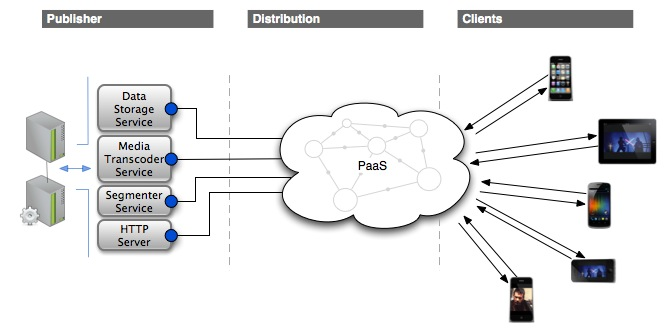
\includegraphics[width=0.9\textwidth]{./Images/cashed5}
\caption{Ecosystem}
\label{fig:cashed}
\end{figure}

Proin auctor lorem at nibh. Curabitur nulla purus, feugiat id, elementum in, lobortis quis, pede. Vivamus sodales adipiscing sapien. Vestibulum posuere nulla eget wisi. Integer volutpat ligula eget enim. Suspendisse vitae arcu. Quisque pellentesque. Nullam consequat, sem vitae rhoncus tristique, mauris nulla fermentum est, bibendum ullamcorper sapien magna et quam. Sed dapibus vehicula odio. Proin bibendum gravida nisl. Fusce lorem. Phasellus sagittis, nulla in hendrerit laoreet, libero lacus feugiat urna, eget hendrerit pede magna vitae lorem. Praesent mauris Class aptent taciti sociosqu ad litora torquent per conubia nostra, per inceptos hymenaeos H.264\slash \ac{AVC} standard, sem vitae rhoncus tristique \ac{SVC} \cite{Fraunhofer-Heinrich-Hertz-Institute:2013fk,ISO:H-264} nulla in hendrerit laoreet, libero lacus feugiat urna, eget hendrerit pede magna vitae lorem.

\textcolor{violet}{You can use in-paragraph lists with this construct for: 
\begin{inparaenum}[(a)]
\item first case;
\item second case; and
\item third case,
\end{inparaenum}
making the text organized and fluid.}

Vivamus auctor leo vel dui. Aliquam erat volutpat. Phasellus nibh. Vestibulum ante ipsum primis in faucibus orci luctus et ultrices posuere cubilia Curae; Cras tempor. Morbi egestas, urna non consequat tempus, nunc arcu mollis enim, eu aliquam erat nulla non nibh. Duis consectetuer malesuada velit. Nam ante nulla, interdum vel, tristique ac, condimentum non, tellus. Proin ornare feugiat nisl. Suspendisse dolor nisl, ultrices at, eleifend vel, consequat at, dolor, morbi egestas, urna non consequat tempus, nunc arcu mollis enim, eu aliquam erat nulla non nibh.

Notice that \gls{maths} makes extensive use of \Glspl{formula}\todo[color=cyan!40, author=RC, fancyline]{example of use of Glossaries}{} which are particularly well rendered in documents produced with \gls{LaTeX}.

Maecenas elementum augue nec nisl. Proin auctor lorem at nibh. Curabitur nulla purus, feugiat id, elementum in, lobortis quis, pede. Vivamus sodales adipiscing sapien. Vestibulum posuere nulla eget wisi. Integer volutpat ligula eget enim. Suspendisse vitae arcu. Quisque pellentesque.
% #############################################################################
\section{Organization of the Document}
This thesis is is organized as follows: \Cref{chap:intro} \todo[color=cyan!40, author=RC, fancyline]{references to doc sections/chapters are automatic}{}interdum vel, tristique ac, condimentum non, tellus. 
In \cref{chap:back} curabitur nulla purus, feugiat id, elementum in, lobortis quis, pede.
In \cref{chap:architecture} consequat ligula nec tortor. Integer eget sem. Ut vitae enim eu est vehicula gravida.
\Cref{chap:implement} morbi egestas, urna non consequat tempus, nunc arcu mollis enim, eu aliquam erat nulla non nibh in \cref{chap:evaluation}.
\Cref{chap:conclusion} suspendisse dolor nisl, ultrices at, eleifend vel, consequat at, dolor.
% If Printing on DOUBLE SIDED pages, the second page should be white.
% Otherwise, comment the following command:
\cleardoublepage
%
%Chapter 2
% #############################################################################
% This is Chapter 2
% !TEX root = ../main.tex
% #############################################################################
% Change the Name of the Chapter i the following line
\fancychapter{Literature Review}
\cleardoublepage
% The following line allows to ref this chapter
\label{chap:back}

%TODO short introduction

This chapter synthesizes the state of the art in causal inference applied to satellite-based environmental monitoring, with a focus on methane (\ch{CH_4}) dynamics. It consolidates methodological advances across five core domains that underpin this thesis: (i) the geophysical behavior and sources of atmospheric methane, (ii) satellite-based retrievals and limitations in current CH\textsubscript{4} products, (iii) statistical causal inference techniques tailored for spatiotemporal environmental data, (iv) the integration of land cover datasets with atmospheric variables, and (v) the baseline empirical analysis by Karoff \& Vara-Vela (2023) \cite{Karoff2023}, which motivates and constrains the present work.

Although existing studies have established robust frameworks for causal inference in economics and biomedicine, only recently have these techniques been adapted for geophysical applications. Within this emerging field, methane has received relatively limited attention despite its critical role in climate feedback loops and its heterogeneous emission sources. This gap is amplified by the challenges of applying causal models to satellite data such as autocorrelation, irregular sampling, and spatial confounding challenges that this research explicitly addresses.

Taken together, the reviewed studies demonstrate a growing interest in applying causal inference to environmental challenges, yet also reveal that methane monitoring from space remains methodologically underserved. The integration of causal analysis with satellite-based observations, particularly when combined with land cover dynamics and atmospheric constituents, remains largely unexplored or limited to correlational approaches. This chapter, therefore, situates the current research within a broader scientific context, highlighting how previous works inform the development of a tailored causal framework for methane attribution. The subsequent sections delve into each component of this interdisciplinary space, providing the necessary foundation for the methodological innovations introduced in the next chapter.


%%%%%%%%%%%%%%%%


\section{Causal Inference Methods for Environmental Time Series}

Traditional environmental analyses have relied on correlation and regression, which cannot distinguish causation from confounding or indirect effects. Judea Pearl's framework for causal inference \cite{Pearl2009} and subsequent advances have enabled the identification of causal relationships from observational data, provided certain assumptions are met.

While remote sensing offers unprecedented data coverage, interpreting complex Earth system relationships requires more than correlation analysis. In time-series analysis, causal inference methods aim to determine whether one variable influences or drives changes in another, moving beyond mere simultaneity. A classical approach is Granger causality (GC), a statistical test introduced by C.W.J. Granger in 1969. In essence, $X$ "Granger-causes" $Y$ if including past values of $X$ significantly improves the prediction of $Y$ compared to using only past $Y$ \cite{Kovacs2023}. In practice, GC is evaluated via predictive linear regression models: if the forecast error of $Y$ is reduced by incorporating lags of $X$, then $X$ is considered a Granger cause of $Y$ (provided certain assumptions like stationarity hold)
\cite{Kovacs2023}. It is important to note that Granger causality, being based on predictability, does not prove a direct physical cause-and-effect; rather, it identifies predictive information flow. Despite this caveat, GC has been widely applied in geosciences as an initial test for directionality in coupled climate variables. For example, recent work by Kovács et al. (2023) \cite{Kovacs2023} employed Granger causality on global satellite indices to untangle drivers of vegetation dynamics. By applying GC analyses pixel-wise between climate variables (like precipitation, temperature) and vegetation indices (NDVI, FAPAR, etc.), they produced global maps of where environmental drivers have causal influence on vegetation anomalies \cite{Kovacs2023}. Such studies demonstrate GC's ability to reveal patterns consistent with known processes (e.g. rainfall Granger-causing vegetation growth in water-limited regions), opening possibilities for improved forecasting \cite{Kovacs2023}. Another pertinent example comes from the paleoclimate realm: Larsson and Persson (2023) \cite{Larsson2023} performed a multivariate Granger causality analysis on 800,000-year ice-core records of temperature, CO$_2$, and CH$_4$. They found strong evidence of bidirectional GC between all three variables, i.e. CO$_2$ Granger-causes temperature and vice versa, and similarly CH$_4$ is both cause and effect in long-term glacial climate feedbacks. This suggests that on geologic timescales, greenhouse gases and temperature mutually reinforce each other in a complex feedback loop. These examples illustrate the utility of Granger causality in climate science, while also reminding us that GC can reflect indirect or common-driver influences (especially when many variables are omitted). 

To capture nonlinear or non-parametric dependencies, information-theoretic measures like Transfer Entropy (TE) have been introduced. Transfer Entropy, proposed by Schreiber (2000) \cite{Schreiber2000}, quantifies the reduction in uncertainty of future $Y$ given knowledge of past $X$ (and past $Y$), effectively measuring the information flow from $X$ to $Y$. Unlike linear GC, transfer entropy can detect nonlinear coupling and does not assume a specific model form. In practice, TE is often estimated through histogram or k-nearest-neighbor methods and requires sufficient data for robust probability distribution estimation. TE has seen growing application in Earth system analysis where relationships may be nonlinear. A noteworthy study by Stips et al. (2016) \cite{Stips2016} used a form of TE (the Liang-Kleeman information flow method \cite{LianKleeman2013}) to investigate the causal links between atmospheric CO$_2$ and global mean temperature \cite{Stips2016}. Their analysis confirmed that, for the modern instrumental period, rising CO$_2$ (and other greenhouse gases) is the causal driver of observed warming, rather than the other way around \cite{Larsson2023}. 

Interestingly, when the same methods were applied to ice-age data, the direction of causality appeared reversed: temperature changes led CO$_2$/CH$_4$ changes, reflecting the slow feedback of carbon cycle processes in paleo-records \cite{Larsson2023}. This example underscores TE's ability to capture directionality in both linear and nonlinear climate interactions. It also highlights the need to interpret causality in context, the causality can be time-scale dependent or mediated by broader system dynamics. More generally, TE and related measures (e.g. conditional mutual information, Rényi transfer entropy) have been used to study topics such as extreme event precursors \cite{Palus2024, Benocci2025}, rainfall dynamics in monsoons \cite{tongal_forecasting_2021}, and even socio-ecological feedbacks \cite{li_integrating_2025}. 

Beyond optimizing computational efficiency for large datasets, recent methodological innovations in causal discovery further strengthen the analytical foundation for rigorously addressing complex environmental challenges like methane attribution. For instance, Cheong et al. \cite{cheong2021causal} demonstrate the power of Structural Causal Models (SCMs) in identifying and correcting for biases. While their specific application was in affect recognition, the core principles of SCMs, involving explicit modeling of confounding structures and the use of structural equations, are highly relevant for disentangling biases and complex dependencies within satellite-derived methane data. 

Similarly, Cheng and Redfern \cite{cheng2021} propose the use of normalized information flow (nIFc) as a robust approach for analyzing high-dimensional Earth system datasets. Their methodology is specifically designed to address challenges analogous to those encountered in methane time series, including complex interdependencies, high noise levels, and sparse observations. These advancements provide more sophisticated tools for unraveling the intricate web of cause-and-effect in environmental systems, moving beyond basic correlative insights.

Recent methodological innovations in causal discovery further strengthen the analytical foundation of this thesis. Cheong et al. \cite{cheong2021causal} demonstrate how structural causal models (SCMs) can be used to identify and correct for bias in affect recognition. While focused on facial expression data, the principles of SCMs, explicit modeling of confounding structures and structural equations are relevant for disentangling biases in satellite, derived methane data. 

Similarly, Cheng and Redfern \cite{cheng2021} propose the use of normalized information flow (nIFc) as a robust approach for quantifying causal contributions in high-dimensional Earth system datasets. Their methodology is specifically designed to provide strong estimates of causal contributions even in challenging situations where standard regressions perform poorly. These situations include cases with significant causal time-lags, substantial noise contributions, alternating feedback (correlation) signs, and complex teleconnections where multiple causes contribute to an overall effect. As exemplified by their analysis of methane-climate feedbacks using both observational data and Earth system models, nIFc offers a powerful means for quantifying nonlinear processes and assessing model performance in contexts directly relevant to methane time series analysis.

Jerzak et al. \cite{jerzak2023} also integrate causal inference on Earth observation data. Their work emphasizes the role of satellite imagery in resolving confounding in observational studies and proposes novel scene-based definitions of treatment and outcome at varying spatial resolutions. These perspectives are especially valuable in methane monitoring, where different processes may operate on spatial scales and resolution mismatches between drivers (e.g., land cover) and outcomes (e.g., XCH\textsubscript{4}) must be causally reconciled.

The CA-SpaceNet framework by Wang et al. \cite{wang_ca-spacenet_2022} offers another example of causal reasoning under complex image-based confounding. Although aimed at space object pose estimation, its use of counterfactual reasoning to reduce background bias parallels the need for bias-resilient causal interpretation in methane remote sensing. 

In the last few years, advanced multivariate causal discovery algorithms have emerged, aiming to unravel complex interdependencies in high-dimensional environmental systems. One prominent example is the PCMCI framework (PCMCI = PC-algorithm for momentary conditional independence), introduced by Runge et al. \cite{Runge2020EGU}. PCMCI combines the classic PC algorithm (which iteratively removes spurious links via conditional independence tests) with a tailored approach for time-lagged data. It performs momentary conditional independence (MCI) tests to identify causal links in specific lags, while accounting for autocorrelation in each time series \cite{Runge2019_2}. This allows PCMCI to handle datasets with many variables and temporal dependencies, typical of Earth system observations. 

In a landmark study, Runge et al. (2019) \cite{Runge2019} demonstrated PCMCI on a dataset with dozens of climate indices and found it could successfully recover known cause-effect relations (like ENSO's influence on Indian monsoon) that simpler correlation or bivariate GC missed \cite{Runge2019, Docquier2024}. 

Subsequent applications in climate science have shown PCMCI's ability to filter out spurious correlations induced by common drivers or autocorrelation, giving a clearer picture of direct causal pathways \cite{Docquier2024}. For instance, Böhnisch et al. (2023) \cite{bohnisch_european_2023} used PCMCI to elucidate the causal network of atmospheric circulation patterns leading to European heat waves, isolating key drivers among many correlated candidates. A recent comparison by Docquier et al. (2024) \cite{Docquier2024} evaluated PCMCI against an information-flow method for North Atlantic climate indices \cite{Docquier2024}. Both methods outperformed simple correlation in identifying true links, with PCMCI excelling when the system involved many variables, thanks to its ability to condition on multiple confounders \cite{Docquier2024}. However, differences emerged in specific link strengths (e.g. one method flagged the Arctic Oscillation as most influential, whereas PCMCI highlighted ENSO) \cite{Docquier2024}. The authors noted that such differences call for further investigation, ideally incorporating nonlinear causal discovery methods in addition to PCMCI's (primarily linear) independence tests \cite{Docquier2024}. This points to an active frontier: hybrid approaches that can capture nonlinearity, handle many variables, and provide confidence measures for causal links in climate data. 

Another important methodological parallel comes from the work of Zhang et al. \cite{zhang_learning_2021}, who developed a bisimulation metric for reinforcement learning that encourages the learning of representations invariant to task-irrelevant details. Although their domain is Markov Decision Processes (MDPs), the core concept—distinguishing signal from noise in high-dimensional environments—translates directly to satellite-based methane analysis. In remote sensing, irrelevant geographic or atmospheric features can obscure causal signals. A causal framework, particularly when used in conjunction with dimensionality-reduction strategies that preserve causal invariants, must be sensitive to these distinctions. The bisimulation approach exemplifies how representation learning techniques can assist in filtering out confounding visual or contextual information in satellite data, potentially enhancing causal interpretability.

In summary, a suite of causal inference tools, from Granger causality and transfer entropy to PCMCI and beyond is now available to probe environmental time series. Each has strengths and weaknesses: GC and pTE offer simplicity and speed but assume linearity (or Gaussianity), whereas TE and information flow capture nonlinearity at the cost of more data and computation, and PCMCI and related algorithms tackle high-dimensional multivariate causality but may miss nonlinear effects. In practice, applying multiple methods in concert can provide complementary insights \cite{Docquier2024, silini_assessing_2023}. The growing literature (especially post-2020) illustrates that these methods, when carefully applied, can successfully disentangle drivers of climate anomalies, ecosystem responses, and other Earth system behaviors that elude standard correlation analysis \cite{Runge2019}. This PhD thesis builds on these developments by applying causal inference to satellite-derived methane time series, a novel combination that leverages the abundant data from remote sensing and the rigor of modern causality frameworks.

Recent years have seen the adaptation of causal discovery methods to environmental time series:
\begin{itemize}
    \item \textbf{Granger causality} \cite{Granger} and its nonlinear extensions have been widely used to infer directional dependencies in climate and ecological data.
    \item \textbf{PCMCI} (Peter and Clark Momentary Conditional Independence) has emerged as a robust method for high-dimensional, autocorrelated time series typical of Earth system datasets \cite{Runge2019}.
    \item \textbf{Transfer entropy} provides a model-free, information-theoretic approach to causality, capturing nonlinear and lagged dependencies \cite{Schreiber2000}.
    \item \textbf{Causality in remote sensing:} \cite{jerzak2023} discuss the challenges and opportunities of integrating Earth observation data into causal inference, highlighting issues such as spatial confounding, measurement error, and the need for domain knowledge.
    \item \textbf{Recent applications:} \cite{Yuan2022} applied causality-constrained machine learning to wetland methane emissions, showing improved interpretability and predictive performance. \cite{Kretschmer2016} and \cite{EbertUphoff2021} demonstrated the utility of causal networks in climate research.
\end{itemize}

Lastly, the increasing integration of machine learning techniques is proving vital for advanced methane monitoring. For instance, Wang et al. \cite{wang2020} developed a machine learning algorithm, leveraging logistic regression, to predict high-emitting sites in the oil and gas sector that could be prioritized for repair. This approach aimed to cost-effectively identify "super-emitters" whose stochastic and intermittent leaks are responsible for a majority of emissions, thereby significantly reducing survey costs and increasing emissions reductions compared to conventional methods.

In the same line, Yuan et al. \cite{Yuan2022} developed a causality-guided machine learning model for wetland \ch{CH4} emissions. This work, using flux measurements from \gls{eddy_covariance} towers, successfully identified consistent causal regulations, such as soil temperature dominating \ch{CH4} emissions across wetland types. The use of ground-level, in-situ devices in such studies is particularly valuable as it allows for a controlled collection of all measured variables, simplifying the co-location and harmonization process, which greatly facilitates robust causal analysis. 

These examples underscore the applicability of causal inference tools beyond climate time series, reinforcing the methodological diversity required to address the methane attribution problem.

\section{Integrating Land Cover, Atmospheric Data, and Causality}
Land cover is a key driver of methane emissions, especially for wetlands, agriculture, and \gls{urban_areas} \cite{Saunois2020, Karoff2023}. MODIS and ESA WorldCover provide global, high-resolution land cover maps that can be integrated with atmospheric data for causal analysis \cite{Friedl2010, Zhang2021}.

A key focus of this research is the integration of land cover information with atmospheric methane data under a causal analysis framework. Land cover and land use have profound effects on methane emissions: for instance, wetlands are the largest natural source of methane, rice paddies and cattle pastures contribute significant agricultural emissions, while urbanized or arid lands emit relatively little CH$_4$. At the same time, atmospheric methane concentrations can feedback on ecosystems (e.g. via climate change). Understanding these interactions requires linking spatio-temporal data on land surface with atmospheric measurements. 

Prior studies have approached this integration mostly through statistical or process-modeling methods rather than explicit causal discovery. One line of research has used remote sensing to connect climate variability, land cover changes, and methane fluxes. Pandey et al. (2017) \cite{Pandey2017} provided an example by examining how an extreme climate event (the 2011 La Ni\~na) impacted wetland extent and thereby methane emissions. They found that anomalously high rainfall during La Ni\~na expanded tropical wetland inundation area, which in turn led to a 5-9 Tg increase in CH$_4$ release, detectable via higher column methane in satellite data. By correlating precipitation anomalies, satellite-derived inundation, and methane observations, their study inferred a possible causal chain: La Ni\~na → increased wetlands → elevated CH$_4$ emissions. Although Pandey et al. did not employ formal causality tests, the evidence strongly suggested that wetlands were the cause of the methane spike (rather than a mere coincidence). This illustrates how multi-source data (climate indices, land cover, gas measurements) can be pieced together to tell a causal story about the Earth system.

At a more local scale, researchers have combined ground-based flux measurements with satellite time series to attribute carbon budget components. In an early study, Yan et al. (2008) \cite{Yan2008} tackled the problem of "closing" the carbon balance in an estuarine wetland by integrating eddy-covariance tower data with MODIS satellite observations. They noted that a simple productivity model severely underestimated the wetland's carbon uptake, hypothesizing that unaccounted methane release and tidal carbon export were causing the discrepancy. By incorporating remote-sensing indicators, a land surface water index (LSWI) for inundation, evapotranspiration (ET) for wetland metabolism, and tidal height, into an autoregressive model of gross primary production (GPP), they significantly improved model performance. The modified model's estimates matched observed net carbon exchange much better ($R^2$ increased from 0.55 to 0.88). Effectively, this approach embedded land surface variables into a time-series prediction, which is closely aligned with causal attribution: it demonstrated that including the effects of water inundation and methane emissions (drivers) was necessary to explain the carbon dynamics. Although Yan et al. did not use the term "causality" their integrated model functioned akin to a causal model, identifying tidal flooding and methane release as drivers of carbon losses that needed to be accounted for. This underscores the value of blending atmospheric data with land cover/phenology data to capture cause-effect relations in biogeochemical cycles.

Most recent studies have also explored data-driven correlations between land use and air quality. Jodhani et al. (2024) \cite{Jodhani2024}, for example, utilized Google Earth Engine to fuse Sentinel-5P pollutant data with land-cover classifications in India. They examined how different LULC categories (urban, agricultural, forest, water, etc.) correspond to variations in gases like CO, NO$_2$, SO$_2$, HCHO, and CH$_4$ over multiple years. Their results showed clear associations for short-lived pollutants (e.g. NO$_2$ hotspots over cities and industrial regions, elevated SO$_2$ near coal power plants). Methane, in contrast, showed a relatively uniform spatial distribution over the region, with no sharp local hotspots. This was attributed to methane's long atmospheric lifetime and well-mixed background, local land use had less immediate impact on column CH$_4$ compared to more regional or global influences. Nonetheless, Jodhani et al. found subtle differences aligned with land cover: for instance, areas of intensive agriculture and wetlands in Gujarat did exhibit slightly higher CH$_4$ concentrations than arid or urban areas (consistent with expected emissions from rice paddies and reservoirs). Studies like this provide a baseline of where methane concentration differences coincide with land surface characteristics. The next step, which our research undertakes, is to rigorously test which differences are causally attributable to land cover as opposed to confounding factors like meteorology or transport.

Integrating land cover data into a causal inference framework for methane involves several strategies. An approach is to stratify the analysis by land cover type. effectively comparing time series of CH$_4$ over different surface categories (wetlands, agriculture, forests, etc.) and testing for lead-lag relationships or causal links between these categories and methane variability. Karoff and Vara-Vela (2023) \cite{Karoff2023} made an initial foray into this by computing separate methane seasonal cycles for each type of land and region. Their study, detailed in Section \ref{sec:baseline}, serves as a baseline for our investigation.

A particularly relevant contribution comes from Jerzak et al. \cite{jerzak2023}, who address the challenge of using satellite imagery as a proxy for confounding variables in causal inference. They discuss the definition of treatment, outcome, and confounder at image scale and examine how resolution mismatches can distort causal estimates. This has strong implications for our integration of land cover (from MODIS/ESA) with methane data (from TROPOMI), where aggregation choices and observational granularity can influence inferred causal links. Their simulation results also guide practical design decisions, such as how kernel bandwidth and pixel size affect bias and variance in estimation.

From a methodological standpoint, integrating land cover in causality analysis often means dealing with spatially distributed time series (maps over time). Techniques like PCMCI have been extended to gridded data, essentially building causal networks in each grid cell and allowing teleconnections between cells \cite{Runge2019, Runge2020EGU}. In our context, rather than analyze every pixel globally (which is computationally prohibitive), we focus on aggregated time series over distinct land cover classes or regions of interest. This retains physical interpretability (e.g. "wetland regions' CH$_4$ vs. upland regions' CH$_4$") while simplifying the causal discovery problem. The literature suggests this approach is promising: for example, Kovács et al. (2023) \cite{Kovacs2023} derived causal links between global biomes and climate drivers by aggregating pixels into biome categories, finding that precipitation Granger-caused vegetation changes most strongly in arid biomes \cite{Kovacs2023}. Analogously, we might find that certain land-cover types (like wetlands) exert a causal influence on methane anomalies (e.g. via episodic release events) whereas others (like deserts) do not, or that the causal effect is mediated by climate variables. 


To our knowledge, no prior study has systematically applied causal discovery algorithms to satellite-based methane time series categorized by land cover, within an automated framework. Thus, our work pioneers this integration, aiming to identify cause-effect relations such as "wetland extent → methane concentration" or "irrigated cropland → methane" in a data-driven way. This fills a gap between remote-sensing studies that correlate CH$_4$ with land surface properties and process-based modeling studies that simulate CH$_4$ emissions given land surface conditions. Using causal methods, we seek to move from correlation to attribution, determining which land cover factors are genuine drivers of methane variability and which observed associations might be spurious or indirectly caused by other factors.


\section{Baseline Study by Karoff \& Vara-Vela (2023)} 
\label{sec:baseline}

The analysis by Karoff and Vara-Vela (2023) \cite{Karoff2023} serves as an important starting point for our research. Their study is a data-driven exploration of how atmospheric methane concentrations vary as a function of geography, land cover type, and season. In many ways, it establishes the empirical patterns and puzzles that a causal study (like ours) needs to explain. Karoff and Vara-Vela compiled three years of TROPOMI Sentinel-5P XCH$_4$ data (2017-2020) and stratified the observations by land cover categories using MODIS and ESA WorldCover datasets. They deliberately processed the methane data with two independent retrieval algorithms (as noted earlier, one of which was likely the WFMD/WFM-DOAS and the other the RemoTeC-based product) to ensure that results were not an artifact of a single retrieval method. The methane measurements were then aggregated over each land cover class (such as croplands, wetlands, forests, shrublands, \gls{savannas}, urban areas, etc.) and analyzed for differences in mean concentration and seasonal cycle.

In general, they observed that the phase of the annual CH$_4$ cycle differs by continent: over croplands, shrublands, and savannas, African sites showed a delayed seasonal peak compared to Asian sites. This hints that regional climatic differences (e.g. timing of wet/dry seasons) modulate methane seasonality depending on land context. A causal analysis could build on this by including climate variables (temperature, precipitation) along with land type as potential causes of the methane seasonal phase shift. Another strategy is using causal graph or network models where nodes include not just CH$_4$ concentration, but also land-surface variables like normalized difference wetness index (for wetlands), burned area (for biomass burning), or anthropogenic activity proxies. By treating land indicators as part of a multivariate causal model, one can ask, for instance: Do changes in wetland extent Granger-cause changes in methane, after controlling for precipitation and temperature? Or Does irrigation expansion (cropland increase) in a region lead to rising CH$_4$ levels, or are both driven by a third factor? There is nascent work in this direction, such as studies linking deforestation to local climate via GC tests \cite{Kovacs2023}, but applying it specifically to methane remains largely unexplored.

The authors' findings reported that, on a global scale, the highest column-average methane tends to occur over agricultural areas, especially croplands, whereas the lowest methane values occur over regions like shrublands. This aligns with expectations: intensive agriculture (including rice paddies and ruminant livestock) is a major anthropogenic methane source, whereas shrublands (often arid or semi-arid) have sparse vegetation and low wetland extent, hence fewer methane emitters. Such a gradient from high CH$_4$ over croplands to low CH$_4$ over shrublands was consistently observed on multiple continents. In contrast, forests and savannas showed intermediate methane levels, and interestingly, urban areas did not stand out as high-methane regions (likely because methane sources in cities are relatively diffuse or small compared to the wide-area averaging of satellite pixels). The most surprising result was that methane concentrations over wetlands were not as high as expected. 

In fact, Karoff \& Vara-Vela found that wetlands exhibited lower than average CH$_4$ concentrations in the satellite data. This is counter-intuitive since wetlands are well-known natural methane sources (due to anaerobic decomposition in waterlogged soils). One would anticipate wetlands to show elevated CH$_4$ column abundance. The authors noted this discrepancy and cautioned that methane measurements from TROPOMI over wetland areas should be "handled with caution" until the cause is understood. They hypothesized that retrieval issues (perhaps related to water, humidity, or aerosol in wetland regions) might be contributing to anomalously low satellite readings, rather than wetlands truly having less methane. This unresolved point directly motivates a deeper investigation, potentially with causal analysis to discern if the low wetland CH$_4$ is a retrieval artifact (instrumental cause) or if there is an actual physical mechanism (e.g. wetlands coinciding with strong OH radical presence that destroys methane, though such an effect would be unusual). Our work will build on this finding by probing it with causal discovery tools, to see if we can detect any systematic "bias" link between wetland fraction and CH$_4$ (which would support the artifact theory) or any external driver that depresses CH$_4$ over wetlands.

In addition to spatial patterns, Karoff \& Vara-Vela examined seasonal variations of methane over different land types. They observed that methane generally has a seasonal cycle (driven by factors like hydroxyl radical seasonality and emissions timing), and this cycle's phase can differ by region. For example, over croplands, shrublands, and savannas in Africa, the annual peak in CH$_4$ occurred later in the year compared to similar land covers in Asia. One interpretation is that African methane sources (and/or transport patterns) are phased differently, possibly related to later wet seasons or biomass burning events in the Southern Hemisphere. While their research paper did not conclusively explain these phase shifts, it highlighted that geographic context matters: the interplay of land cover with regional climate leads to unique methane timing signatures. This again suggests the presence of underlying causal factors (monsoonal rains, temperature cycles, etc.) that differ between continents. Karoff \& Vara-Vela's study was intentionally kept data-driven and non-causal, they mapped and described patterns, without formally attributing causes. They emphasized known expectations (like cropland vs shrubland differences) and flagged anomalies (like the wetlands issue), but stopped short of testing hypotheses about why those patterns occur. In their conclusion, they specifically pointed out the wetland methane discrepancy as an open question. They also mentioned that until such discrepancies are resolved, one should be careful in using the data for emission quantification. This cautious approach underscores the need for further analysis, precisely what our thesis aims to do by applying causal inference techniques.

In summary, the Karoff \& Vara-Vela (2023) study provides a valuable benchmark of methane distribution across land covers, against which we can compare our causal analysis results. It represents the state-of-the-art in pure statistical description of satellite methane data. Our work extends this by inferring directionality and drivers: for instance, where they noted high CH$_4$ over croplands, we will investigate whether cropland extent Granger-causes methane increases (indicating emissions effect) or if the correlation could be due to a third factor. Where they found the puzzling wetland low bias, we will use causal methods to test potential explanations (such as a hidden variable like aerosol optical depth affecting the retrievals). In doing so, we treat Karoff \& Vara-Vela's results as the foundation, a non-causal baseline, upon which a causal understanding will be built. This progression from description to causation exemplifies the evolution of scientific inquiry in this domain. By positioning their study as the baseline, we ensure that our advanced analyses remain grounded in the empirical reality of the observations, and we directly address the gaps they identified.


\section{Knowledge Gaps, Challenges, and Research Opportunities}

Reviewing the literature reveals several critical knowledge gaps at the intersection of satellite methane observation, land cover characterization, and causal analysis. First, while numerous studies have leveraged satellite data to correlate methane with land surface features or external drivers (ENSO events, seasonal cycles, etc.), very few have applied formal causal inference techniques to these datasets. The years 2020-2024 saw a surge in Earth science causality research \cite{Runge2019}, yet applications have mostly centered on climate indices or model outputs, not on remotely-sensed greenhouse gas measurements. In particular, there is a lack of studies that take the rich spatiotemporal record of methane from TROPOMI and ask causally (e.g., what drives the observed variations and trends across different landscapes). 

The baseline analysis by Karoff \& Vara-Vela (2023) \cite{Karoff2023} is emblematic as this mapped differences but did not attribute cause nor formal correlationships. As a result, some observations are unexplained (e.g. wetlands show anomalously low CH$_4$). Is it a data artifact?, or could it be that wetlands, perhaps being largely remote and clean-air sites, coincide with conditions that favor methane oxidation (for instance, higher UV leading to more OH radicals)?. To date, no studies have conclusively answered this question. A targeted causal analysis could test hypotheses by including potential explanatory variables (such as retrieval parameters, cloud cover, \ch{OH} concentration proxies) to see if they explain the wetland anomaly.

Another gap lies in understanding spatiotemporal variability of methane in relation to land cover changes. We know qualitatively that if, say, wetlands expand, methane emissions likely rise, and if wetlands dry up or are drained, emissions fall. However, this has rarely been demonstrated with observational data in a causal sense. The Pandey et al. (2017) \cite{Pandey2017} study gave one example with ENSO-driven wetland expansion, but such events are rare. More common are gradual land use changes, for instance, agricultural expansion, urban sprawl, or natural wetland loss; happening continuously around the globe. Do these changes leave a discernible fingerprint in atmospheric methane growth rates regionally? If so, can we detect it with Granger causality or PCMCI by linking land cover time series to methane time series? This remains an open question. 


The current literature on land-atmosphere causal links has focused more on CO$_2$ (for example, deforestation effects on local climate) or on weather extremes and land cover \cite{Kovacs2023}. Methane, being a less abundant but more potent greenhouse gas, has not received the same causal scrutiny. With new data available (e.g. annual land cover maps from MODIS or Copernicus and daily methane maps from TROPOMI), we are now in a position to investigate these links. A potential outcome could be identifying "hotspots" where land use change is actually causing detectable methane concentration changes (e.g., rapid irrigation development causing more rice paddies and thus methane, or conversely, wetland restoration reducing methane if the restored wetlands are managed in a certain way).

%%%%%%%%%% finished here
A further gap is methodological: bridging the scales between local process studies and global satellite analysis. Many causal inference techniques (including PCMCI, TE) were originally developed for well-defined time series (like climate indices or station data). Applying them to gridded satellite data involves challenges like high dimensionality, autocorrelation across space, and the confounding effect of atmospheric transport that mixes signals from different regions. The Nature Communications perspective by Runge et al. (2019) \cite{Runge2019} emphasizes the need to tailor causal discovery methods to Earth science data, warning that naive application can lead to misinterpretation \cite{Runge2019}. The community has responded by creating platforms like CauseMe.net \cite{Runge2019, Runge2019_2, MunozMari2020} for benchmarking methods on realistic datasets. However, in the specific context of methane and land cover, there is virtually no prior art, meaning we must navigate issues like choosing appropriate spatial aggregation (to avoid unwieldy variable counts), detrending for seasonal cycles (to avoid spurious causality from common trends), and ensuring the data meet assumptions of the causal tests (e.g. approximate stationarity after removing known trends). Our literature review did not find any study that has attempted PCMCI or Granger tests on, say, time series of "methane over forests" vs "methane over croplands" or similar. This represents a methodological gap our work aims to fill, by developing a framework for such analysis.

Another knowledge gap highlighted by the literature is the interpretation of causality in complex systems. Even when causal links are identified, making physical sense of them can be challenging. For example, Docquier et al. (2024) \cite{Docquier2024} found differing causal drivers for climate indices depending on the method \cite{Docquier2024}. In our context, suppose we find that "cropland fraction Granger-causes methane" in certain regions. We must interpret whether this truly means agricultural emissions are driving methane increases (which is plausible), or whether cropland fraction is acting as a proxy for some other factor (e.g. human population or industrial activity that co-occurs with croplands). Similarly, if we find no causal link for wetlands, does that mean wetlands don't influence atmospheric methane? Or could it be that the satellite data's noise masks the link, or that the causal effect is non-linear (e.g. only when wetlands exceed a certain inundation threshold do emissions spike, which a linear test might miss)? These nuances imply a gap between statistical causality detection and domain understanding. The literature suggests combining domain knowledge with data-driven results to avoid misattribution \cite{silini_assessing_2023, Runge2019}. In our thesis, we plan to address this by cross-checking causal findings with independent evidence (e.g. emission inventories, known event timelines like droughts or floods, etc.). For instance, if a causal analysis flags a particular land cover as a driver of methane in a region, we will verify whether known emission inventory data or field studies support that. This step is necessary to translate the quantitative causal discovery into credible scientific conclusions.

Finally, the confluence of these topics (satellite methane, land cover, and causality) points to a gap in practical applications for climate change mitigation. Satellites like Sentinel-5p were designed not just for science but also to support emissions mitigation by identifying sources. To date, most efforts in that vein have focused on pinpointing "super-emitters" (e.g. major gas leaks) via remote sensing. The broader question of causal attribution (e.g. which sectors or land uses are most responsible for observed methane increases) is often addressed using bottom-up inventories or inverse modeling, rather than direct data-driven causality analysis. Our literature survey indicates that applying causal inference directly on observations could provide a complementary, data-driven perspective to these top-down model studies. For example, if agricultural land expansion in South Asia is causally linked with methane increases, this reinforces inventory-based attributions and could sharpen policy focus. Conversely, if certain wetland regions show rising methane that is not causally explained by local temperature or precipitation changes, it might hint at unaccounted anthropogenic inputs or biases. Such insights would be highly relevant to closing the global methane budget, which still has uncertainties (often termed the "methane enigma" for the post-2007 renewed rise). By identifying which variables and regions play a causal role, we contribute to narrowing those knowledge gaps.

% TODO: Merge the section with the following:
Despite notable progress in applying causal analysis to Earth observation data, significant research gaps and methodological challenges remain challenges that our work directly aims to address:

\paragraph{Focus on Correlation over Causation:} 
Most prior studies in methane remote sensing and climate data analysis focus on identifying correlations or temporal trends, without conclusively establishing causal relationships. There is a lack of systematic causal inference applied specifically to methane observations, a gap this study addresses by centering the analysis on explicit cause-effect questions rather than descriptive associations.

\paragraph{Limited Integration of Data Sources.} 
Few existing works integrate multiple satellite products and land surface data within a unified causal framework. Typically, studies examine one dataset or one potential driver at a time. In contrast, our approach simultaneously considers multiple atmospheric variables (e.g., \ch{CO}, \ch{NO2}), land cover types, and meteorological context. This enables us to uncover multifactor causal networks, such as how land cover might modulate the influence of temperature on methane levels. Such data fusion is relatively novel and allows for the discovery of interactions that single-source analyses may overlook.

\paragraph{Handling of Confounding and Autocorrelation:} 
Many existing studies insufficiently address key methodological issues, such as confounding factors, autocorrelation in time series, and the multiple comparisons problem. Climate studies often rely on simple lag correlations, which can be misleading if autocorrelation is not properly accounted for, or if multiple lags are tested without correction. We explicitly incorporate techniques to address these issues: multivariate testing for confounding, autocorrelation-aware methods such as PCMCI, and statistical correction procedures like false discovery rate (FDR) control. This rigorous methodology aims to reduce false positives and increase confidence in the robustness of inferred causal links.

\paragraph{Reproducibility and Open Tools:} 
There is a marked lack of reproducible and openly available workflows for causal inference in the context of environmental remote sensing. Much of the work in this area relies on bespoke scripts that are not easily generalizable or reusable. This represents a clear opportunity for methodological innovation. A core contribution of our project is the development and publication of an open-source causal analysis framework, complete with code and documentation, which can be adopted or extended by other researchers. By promoting transparency and reuse, this work moves the community toward more standardized and collaborative practices in causal inference for Earth system science.

\medskip

By identifying and targeting these research gaps, our project clarifies key opportunities for advancing the field. It will demonstrate how moving from correlation to causation can yield deeper scientific insights, for example, by distinguishing true drivers of methane variability from spurious associations. It will also illustrate the power of data fusion: integrating atmospheric and land surface data under a causal lens to uncover previously unrecognized mechanisms (e.g., specific land cover classes exerting influence on methane seasonal amplitudes). Finally, by openly sharing our framework, we aim to catalyze further research, enabling its application to other greenhouse gases or environmental processes and thereby amplifying the scientific impact of our work beyond the specific case of methane.

In conclusion, this literature review underscores the novelty and importance of our research focus. The gaps define the frontier that this work aims to push forward. Through careful synthesis of recent advances and foundational studies, we have formulated a research approach that uses state-of-the-art causal inference to tackle open questions left by prior data-driven analyses. The ensuing chapters will detail our methodology to address these gaps and will compare our findings against the expectations and puzzles drawn from the literature. In doing so, we hope to contribute both to a new scientific understanding of methane dynamics and a demonstration of how modern causal tools can be applied in Earth observation research \cite{Runge2019}.

%%%%%




% If Printing on DOUBLE SIDED pages, the second page should be white.
% Otherwise, comment the following command:
\cleardoublepage
%
%Chapter 3
% #############################################################################
% This is Chapter 3
% !TEX root = ../main.tex
% #############################################################################
% Change the Name of the Chapter i the following line
\fancychapter{This is the Third Chapter}
\cleardoublepage
% The following line allows to ref this chapter
\label{chap:architecture}

Donec gravida posuere arcu. Nulla facilisi. Phasellus imperdiet. Vestibulum at metus. Integer euismod. Nullam placerat rhoncus sapien. Ut euismod. Praesent libero. Morbi pellentesque libero sit amet ante. Maecenas tellus. Maecenas erat. Pellentesque habitant morbi tristique senectus et netus et malesuada fames ac turpis egestas.
% #############################################################################
\section{Architecture Design} 
\textcolor{violet}{Example of a Flowchart for a system, in \Cref{fig:flowchart}, created with \url{https://app.diagrams.net} and then exported as ``PDF'' crop format (a true vector image that can be scaled to no end, with no pixels or distortion).}

\begin{figure}[h]
\centering
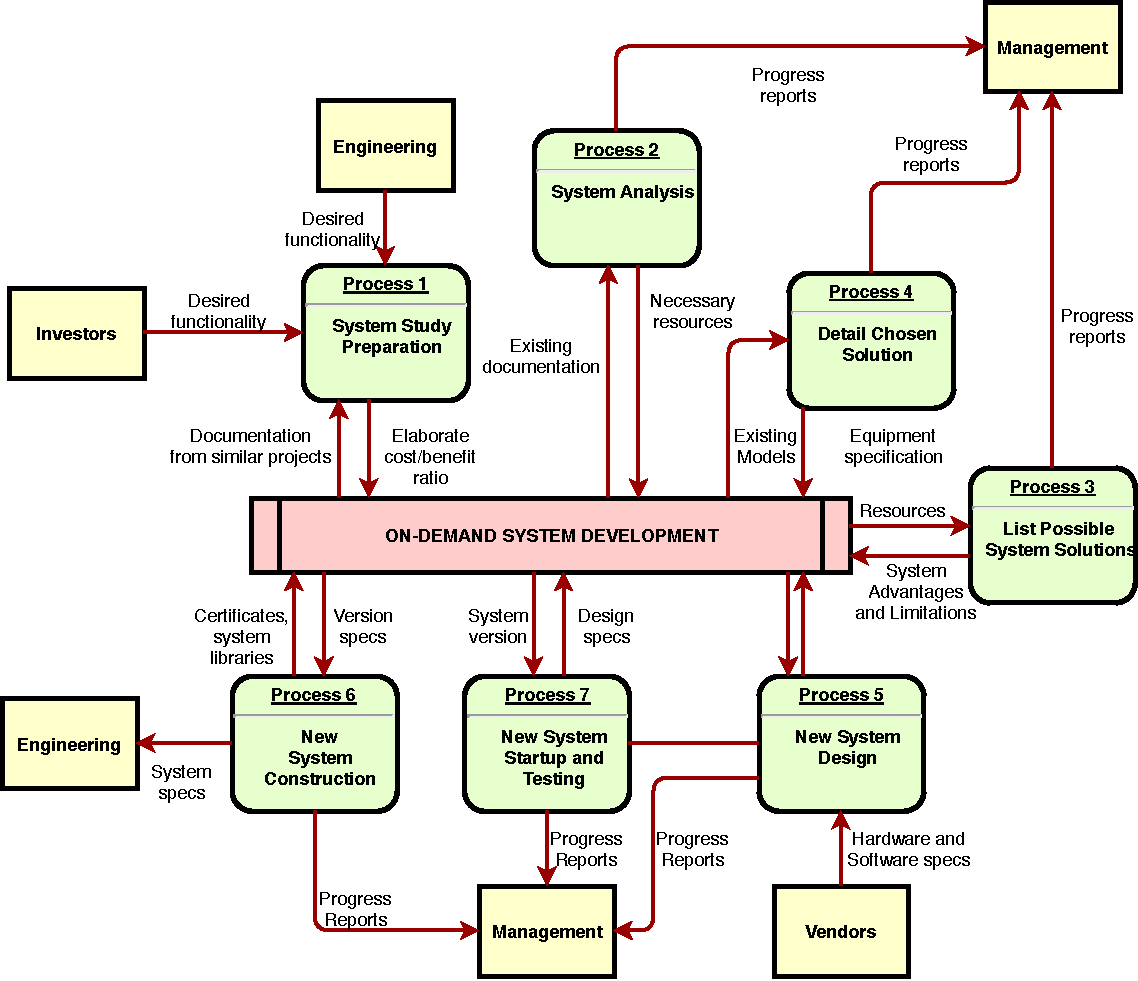
\includegraphics[width=1.0\textwidth]{./Images/Flowchart_from_draw-io.pdf}
\caption{System Processes}
\label{fig:flowchart}
\end{figure}

Quisque facilisis erat a dui. Nam malesuada ornare dolor. Cras gravida, diam sit amet rhoncus ornare, erat elit consectetuer erat, id egestas pede nibh eget odio. Proin tincidunt, velit vel porta elementum, magna diam molestie sapien, non aliquet massa pede eu diam. Aliquam iaculis. Fusce et ipsum et nulla tristique facilisis. Donec eget sem sit amet ligula viverra gravida. Etiam vehicula urna vel turpis. 

\textcolor{violet}{And here another diagram of a network (\Cref{fig:network}) created with \url{https://app.diagrams.net} and then exported as ``PDF'' crop format.}

\begin{figure}[h]
\centering
\includegraphics[width=1.0\textwidth]{./Images/Network_from_draw-io.pdf}
\caption{Network Diagram}
\label{fig:network}
\end{figure}

Suspendisse sagittis ante a urna. Morbi a est quis orci consequat rutrum. Nullam egestas feugiat felis. Integer adipiscing semper ligula. Nunc molestie, nisl sit amet cursus convallis, sapien lectus pretium metus, vitae pretium enim wisi id lectus. Donec vestibulum. Etiam vel nibh. Nulla facilisi. Mauris pharetra. Donec augue. Fusce ultrices, neque id dignissim ultrices, tellus mauris dictum elit, vel lacinia enim metus eu nunc:

\begin{description}
	\item[\textbf{Web-streaming:}]
	The client application should support streaming media using \ac{HTTP} protocols.
	\item[\textbf{Multi-source streaming:}]
	The client application should support multi-source streaming media, i.e., ``simultaneous'' streaming of media content components from a network, supported\slash complemented by \ac{CDN}\slash \ac{CC} services. 
	\item[\textbf{Support content Metadata Description:}]
	The client application should support content metadata description in a format similar or compliant with MPEG \ac{DASH} \cite{ISO/IEC:2012fk}. 
	\item[\textbf{Scalable and Adaptive Media Contents:}]
	The system should support on-demand streaming of scalable and adaptive contents based on \ac{SVC}.
	\item[\textbf{Heterogenous End-User Devices:}]
	The client application should be compatible with current and future generations of end-user devices form factors, irrespective of their performance, screen size and resolution.
	\item[\textbf{Access Network independency:}] 
	The solution should provide the expected service over different types of access networks supported by the end-user devices, such as Wireless \acp{LAN} (IEEE 802.11) or cellular data networks such as \ac{GPRS}, \ac{UMTS}, \ac{LTE}, etc.
\end{description}

Cras gravida, diam sit amet rhoncus ornare, erat elit consectetuer erat, id egestas pede nibh eget odio. Proin tincidunt, velit vel porta elementum, magna diam molestie sapien, non aliquet massa pede eu diam. Aliquam iaculis. Fusce et ipsum et nulla tristique facilisis.
% #############################################################################
\section{Architecture Design Requirements}
Ut nulla. Vivamus bibendum, nulla ut congue fringilla, lorem ipsum ultricies risus, ut rutrum velit tortor vel purus. In hac habitasse platea dictumst. Duis fermentum, metus sed congue gravida, arcu dui ornare urna, ut imperdiet enim odio dignissim ipsum. Nulla facilisi. Cras magna ante, bibendum sit amet, porta vitae, laoreet ut, justo. Nam tortor sapien, pulvinar nec, malesuada in, ultrices in, tortor. Cras ultricies placerat eros. Quisque odio eros, feugiat non, iaculis nec, lobortis sed, arcu. Pellentesque sit amet sem et purus pretium consectetuer \Cref{mpd}\todo[color=cyan!40, author=RC, fancyline]{A listing for XML code, with syntax highlighting}{}.

\begin{minipage}[c]{0.95\textwidth}
\begin{center}
\begin{spacing}{0.5}
\begin{lstlisting}[frame=lines,style=XML,caption={Example of a MPD file.},label=mpd]
<?xml version="1.0" encoding="UTF-8"?>
<StreamInfo version="2.0">
    <Clip duration="PT01M0.00S">
        <BaseURL>videos/</BaseURL>
        <Description>svc_1</Description>
        <Representation mimeType="video/SVC" codecs="svc" frameRate="30.00" bandwidth="401.90"
            width="176" height="144" id="L0">
            <BaseURL>svc_1/</BaseURL>
            <SegmentInfo from="0" to="11" duration="PT5.00S">
                <BaseURL>svc_1-L0-</BaseURL>
            </SegmentInfo>
        </Representation>
        <Representation mimeType="video/SVC" codecs="svc" frameRate="30.00" bandwidth="1322.60"
            width="352" height="288" id="L1">
            <BaseURL>svc_1/</BaseURL>
            <SegmentInfo from="0" to="11" duration="PT5.00S">
                <BaseURL>svc_1-L1-</BaseURL>
            </SegmentInfo>
        </Representation>
    </Clip>
</StreamInfo>
\end{lstlisting}
\end{spacing}
\end{center}
\end{minipage}

Nam malesuada ornare dolor. Cras gravida, diam sit amet rhoncus ornare, erat elit consectetuer erat, id egestas pede nibh eget odio. Proin tincidunt, velit vel porta elementum, magna diam molestie sapien, non aliquet massa pede eu diam.
% If Printing on DOUBLE SIDED pages, the second page should be white.
% Otherwise, comment the following command:
\cleardoublepage
%
%Chapter 4
% #############################################################################
% This is Chapter 4
% !TEX root = ../main.tex
% #############################################################################
% Change the Name of the Chapter i the following line
\fancychapter{This is the Fourth Chapter}
\cleardoublepage
% The following line allows to ref this chapter
\label{chap:implement}

Aliquam aliquet, est a ullamcorper condimentum, tellus nulla fringilla elit, a iaculis nulla turpis sed wisi. Fusce volutpat. Etiam sodales ante id nunc. Proin ornare dignissim lacus. Nunc porttitor nunc a sem. Sed sollicitudin velit eu magna. Aliquam erat volutpat. Vivamus ornare est non wisi. Proin vel quam. Vivamus egestas. Nunc tempor diam vehicula mauris. Nullam sapien eros, facilisis vel, eleifend non, auctor dapibus, pede. 
% #############################################################################
\section{Development Process}
Suspendisse vestibulum dignissim quam. Integer vel augue. Phasellus nulla purus, interdum ac, venenatis non, varius rutrum, leo. Pellentesque habitant morbi tristique senectus et netus et malesuada fames ac turpis egestas. Duis a eros. Class aptent taciti sociosqu ad litora torquent per conubia nostra, per inceptos hymenaeos. Fusce magna mi, porttitor quis, convallis eget, sodales ac, urna. Phasellus luctus venenatis magna. Vivamus eget lacus. Nunc tincidunt convallis tortor. Duis eros mi, dictum vel, fringilla sit amet, fermentum id, sem. Phasellus nunc enim, faucibus ut, laoreet in, consequat id, metus. Vivamus dignissim. Cras lobortis tempor velit. Phasellus nec diam ac nisl lacinia tristique. Nullam nec metus id mi dictum dignissim. Nullam quis wisi non sem lobortis condimentum. Phasellus pulvinar, nulla non aliquam eleifend, tortor wisi scelerisque felis, in sollicitudin arcu ante lacinia leo.:

\begin{itemize}
\item{Technology Research and Related Works}
\item{Requirements Gathering and Study}
\item{Design of the Architecture}
\item{Implementation Process}
\item{Testing and Functional Validation}
\end{itemize}

Pellentesque nibh felis, eleifend id, commodo in, interdum vitae, leo. Praesent eu elit. Ut eu ligula. Class aptent taciti sociosqu ad litora torquent per conubia nostra, per inceptos hymenaeos. Maecenas elementum augue nec nisl. Proin auctor lorem at nibh. Curabitur nulla purus, feugiat id, elementum in, lobortis quis, pede. Vivamus sodales adipiscing sapien. Vestibulum posuere nulla eget wisi. Integer volutpat ligula eget enim. Suspendisse vitae arcu. Quisque pellentesque. Nullam consequat, sem vitae rhoncus tristique, mauris nulla fermentum est, bibendum ullamcorper sapien magna et quam. Sed dapibus vehicula odio. Proin bibendum gravida nisl. Fusce lorem. Phasellus sagittis, nulla in hendrerit laoreet, libero lacus feugiat urna, eget hendrerit pede magna vitae lorem. Praesent mauris.
% #############################################################################
\section{Development Environment}
Cras sed ante. Phasellus in massa. Curabitur dolor eros, gravida et, hendrerit ac, cursus non, massa. Aliquam lorem. In hac habitasse platea dictumst. Cras eu mauris \Cref{time_control_algorithm}\todo[color=cyan!40, author=RC, fancyline]{Notice the reference to the Algorithm construct}{}. Quisque lacus. Donec ipsum. Nullam vitae sem at nunc pharetra ultricies. Vivamus elit eros, ullamcorper a, adipiscing sit amet, porttitor ut, nibh. 

\begin{algorithm}[ht]
\DontPrintSemicolon
\Begin{
$nextBitrate \longleftarrow nextDownloadLevel$\;
$nextBitrate \longleftarrow GetNextBitrate()$\;
$cpuLoad \longleftarrow GetCpuLoad()$\;
$bitrateDelta \longleftarrow getBitrateDelta(currentBitrate, nextBitrate)$\;
\BlankLine
\If{$bitrateDelta > maxThreshold$}{
     $SetBitrate(nextBitrate)$\;
   }
\BlankLine
  \If{$minThreshold < bitrateDelta < maxThreshold$ {\bf and} $numAttemps < 2$}{ 
       $numAttemps \longleftarrow numAttemps + 1$\;
       }{
       \uElseIf{$minThreshold < bitrateDelta < maxThreshold$ {\bf and} $numAttemps = 2$}{
       $numAttemps \longleftarrow 0$\;
       }
       \Else{$SetBitrate(nextBitrate)$}
      }
  \If{$0 < bitrateDelta < minThreshold$ {\bf and} $numAttemps < 3$}{
       $numAttemps \longleftarrow numAttemps + 1$\;
       }{
       \uElseIf{$0 < bitrateDelta < minThreshold$ {\bf and} $numAttemps = 3$}{
       $SetBitrate(nextBitrate)$\;
       }
       }
}
\caption{Time Control Strategy}
\label{time_control_algorithm}
\end{algorithm}


Maecenas adipiscing mollis massa. Nunc ut dui eget nulla venenatis aliquet. Sed luctus posuere justo. Cras vehicula varius turpis. Vivamus eros metus, tristique sit amet, molestie dignissim, malesuada et, urna..
% #############################################################################
\section{Client Application}
Cras sed ante. Phasellus in massa. Curabitur dolor eros, gravida et, hendrerit ac, cursus non, massa. Aliquam lorem. In hac habitasse platea dictumst. Cras eu mauris. Quisque lacus. Donec ipsum. Nullam vitae sem at nunc pharetra ultricies. 

Vivamus elit eros, ullamcorper a, adipiscing sit amet, porttitor ut, nibh. Maecenas adipiscing mollis massa. Nunc ut dui eget nulla venenatis aliquet. Sed luctus posuere justo. Cras vehicula varius turpis. Vivamus eros metus, tristique sit amet, molestie dignissim, malesuada et, urna.

Quisque lacus. Donec ipsum. Nullam vitae sem at nunc pharetra ultricies. Cras vehicula varius turpis.



\begin{minipage}[c]{1.0\textwidth}
%\begin{center}
\centering
\begin{lstlisting}[language = C++, numbers = none, escapechar = !,
    basicstyle = \ttfamily\bfseries, linewidth = .6\linewidth, frame=tb, caption={A listing with a Tikz picture overlayed}, captionpos=b, label=tikzlist] 
 int!
   \tikz[remember picture] \node [] (a) {};
 !puissance!
   \tikz[remember picture] \node [] (b) {};
 !(int x,!
   \tikz[remember picture] \node [] (c){};
 !int n) { 

     int i, p = 1; !\tikz[remember picture] \node [] (d){};!           

     for (i = 1; i <= n; i++) 
       p = p * x; !\tikz[remember picture] \node [inner xsep = 40pt] (e){};! 

     return p; !
       \tikz[remember picture] \node [] (f){};!  
 }
\end{lstlisting}

\begin{tikzpicture}[remember picture, overlay,
    every edge/.append style = { ->, thick, >=stealth,
                                  darkgray, dashed, line width = 1pt },
    every node/.append style = { align = center, minimum height = 10pt,
                                 font = \bfseries, fill= green!20},
                  text width = 2.5cm ]
  \node [above left = .75cm and -.75 cm of a,text width = 2.2cm]
                             (A) {return value type};
  \node [right = 0.25cm of A, text width = 1.9cm]
                             (B) {function name};
  \node [right = 0.5cm of B] (C) {list of formal parameters};
  \node [right = 4.cm of d]  (D) {local variables declaration};
  \node [right = 2.cm of e]  (E) {instructions};
  \node [right = 5.cm of f]  (F) {instruction \texttt{\bfseries return}};  
  \draw (A.south) + (0, 0) coordinate(x1) edge (x1|-a.north);
  \draw (B.south) + (0, 0) coordinate(x2) edge (x2|-b.north);
  \draw (C.south) + (0, 0) coordinate(x3) edge (x3|-c.north);
  \draw (D.west) edge (d.east) ;
  \draw (E.west) edge (e.east) ;  
  \draw (F.west) edge (f.east) ;
\end{tikzpicture}
%\end{center}
\end{minipage}

\textcolor{violet}{And here another method (\Cref{tikzlist}) for mixing (overlay) a picture with a listing of code.}
% #############################################################################
\subsection{User Interface}
Donec semper turpis sed diam. Sed consequat ligula nec tortor. Integer eget sem. Ut vitae enim eu est vehicula gravida. Morbi ipsum ipsum, porta nec, tempor id, auctor vitae, purus. Pellentesque neque. Nulla luctus erat vitae libero. Integer nec enim. Phasellus aliquam enim et tortor. Quisque aliquet, quam elementum condimentum feugiat, tellus odio consectetuer wisi, vel nonummy sem neque in elit. Curabitur eleifend wisi iaculis ipsum. Pellentesque habitant morbi tristique senectus et netus et malesuada fames ac turpis egestas. In non velit non ligula laoreet ultrices. Praesent ultricies facilisis nisl. Vivamus luctus elit sit amet mi. Phasellus pellentesque, erat eget elementum volutpat, dolor nisl porta neque, vitae sodales ipsum nibh in ligula. Maecenas mattis pulvinar diam. Curabitur sed leo..

Cras eu mauris. Quisque lacus. Donec ipsum. Nullam vitae sem at nunc pharetra ultricies. Vivamus elit eros, ullamcorper a, adipiscing sit amet, porttitor ut, nibh. Maecenas adipiscing mollis massa. Nunc ut dui eget nulla venenatis aliquet. Sed luctus posuere justo. Cras vehicula varius turpis. 
% #############################################################################
\subsection{Vivamus luctus elit sit amet mi}
Nulla facilisi. In vel sem. Morbi id urna in diam dignissim feugiat. Proin molestie tortor eu velit. Aliquam erat volutpat. Nullam ultrices, diam tempus vulputate egestas, eros pede varius leo, sed imperdiet lectus est ornare odio. Lorem ipsum dolor sit amet, consectetuer adipiscing elit. Proin consectetuer velit in dui. Phasellus wisi purus, interdum vitae, rutrum accumsan, viverra in, velit. Sed enim risus, congue non, tristique in, commodo eu, metus. Aenean tortor mi, imperdiet id, gravida eu, posuere eu, felis. 

Mauris sollicitudin, turpis in hendrerit sodales, lectus ipsum pellentesque ligula, sit amet scelerisque urna nibh ut arcu. Aliquam in lacus. 

\Cref{fig:ui_playout,fig:ui_loading}\todo[color=cyan!40, author=RC, fancyline]{A figure with Subfigures}{} proin at eros non eros adipiscing mollis.

\begin{figure}[htbp]
	\centering
	\subfigure[Media Loading Window]{\label{fig:ui_loading} 		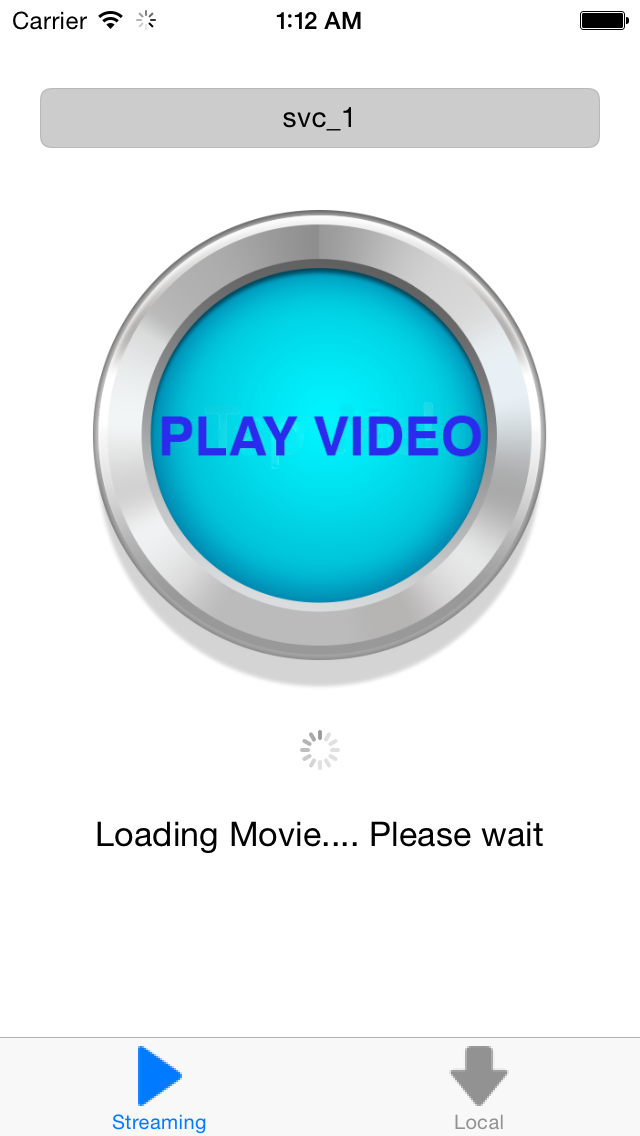
\includegraphics[width=0.3\textwidth]{./Images/ui_loading}} \qquad
	\subfigure[Play-out Session UI]{\label{fig:ui_playout}
		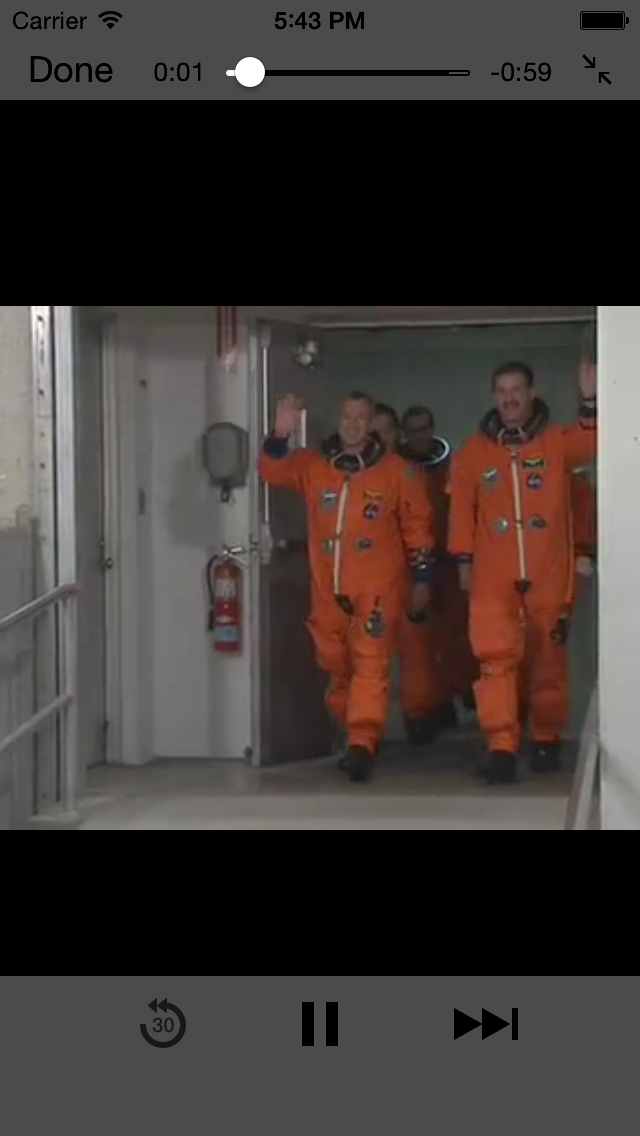
\includegraphics[width=0.3\textwidth]{./Images/ui_playout}}
	\caption{Complete User Interface}
	\label{fig:user_interface}
\end{figure}

Vestibulum ante ipsum primis in \ac{UI} faucibus orci luctus et ultrices posuere cubilia Curae; Nulla placerat aliquam wisi. Mauris viverra odio. Quisque fermentum pulvinar odio. Proin posuere est vitae ligula. Etiam euismod. Cras a eros.
% If Printing on DOUBLE SIDED pages, the second page should be white.
% Otherwise, comment the following command:
%\cleardoublepage
%
%Chapter 5

\fancychapter{Research Plan}
\cleardoublepage
% The following line allows to ref this chapter
\label{chap:evaluation}

%%%%%
\section{Research Plan and Timeline}

This section outlines the structured timeline for the doctoral research, delineating key technical milestones and deliverables from the current year onward. The progression is designed to support the main objective of advancing methane monitoring through causal machine learning applied to satellite time series, with an initial focus on reproducing and extending the methodology developed by Karoff and Vara-Vela \cite{Karoff2023}. The research plan integrates the development of high-performance computing workflows for data preprocessing, systematic implementation of causality testing methods, and the generation of policy-relevant outputs. Each year is articulated in terms of its scientific focus, associated computational or methodological implementations, and expected outputs that contribute incrementally to the overall thesis.


\renewcommand{\arraystretch}{1.3}
\begin{longtable}{@{} >{\centering\arraybackslash}p{3cm} >{\centering\arraybackslash}p{8cm} >{\centering\arraybackslash}p{3cm} @{}}
\caption{Planned milestones, activities, and deliverables across the PhD timeline.}
\label{tab:phd_milestones} \\
\toprule
\textbf{Year} & \textbf{Milestones and Activities} & \textbf{Deliverables} \\
\midrule
\endfirsthead

\toprule
\textbf{Year} & \textbf{Milestones and Activities} & \textbf{Deliverables} \\
\midrule
\endhead

\midrule
\multicolumn{3}{r}{\small\textit{Table~\ref{tab:phd_milestones} continued on next page}} \\
\midrule
\endfoot

\bottomrule
\endlastfoot

\textbf{Year 2 (current)} & 
\begin{minipage}[t]{8cm}\centering
\begin{itemize}[left=0pt, labelsep=4pt, itemsep=2pt]
    \item Continue the curricular courses.
    \item Deploy and adapt methane data extraction scripts for large-scale NetCDF processing using Deucalion HPC.
    \item Integrate MODIS-derived land cover data with TROPOMI-based methane estimates.
    \item Implement and validate statistical pipelines for XCH$_4$ seasonal aggregation and land cover-specific visualizations.
    \item Submit the CAT (Candidature and Thesis) document to the Examination Committee.
\end{itemize}
\end{minipage} &
\begin{minipage}[t]{3cm}\centering
\begin{itemize}[left=0pt, labelsep=4pt, itemsep=2pt]
    \item Operational preprocessing pipeline for WFMD and MODIS data.
    \item Preliminary heatmaps and histograms for seasonal/land cover variation in XCH$_4$.
    \item CAT document.
\end{itemize}
\end{minipage} \\

\addlinespace[0.8em]
\textbf{Year 3} & 
\begin{minipage}[t]{8cm}\centering
\begin{itemize}[left=0pt, labelsep=4pt, itemsep=2pt]
    \item Complete the curricular courses.
    \item Fully reproduce the Karoff and Vara-Vela study, extending to additional land cover classes.
    \item Improve causal discovery techniques: Granger causality, Transfer Entropy, and PCMCI.
    \item Compare causality metrics for spatial-temporal robustness.
    \item Apply multiple-comparison corrections across grid cells and covariates.
    \item Prepare figures and manuscript structure for first peer-reviewed article.
\end{itemize}
\end{minipage} &
\begin{minipage}[t]{3cm}\centering
\begin{itemize}[left=0pt, labelsep=4pt, itemsep=2pt]
    \item Validated causal analysis pipeline (Python/Notebook-based).
    \item Submission of a conference abstract and presentation.
\end{itemize}
\end{minipage} \\

\addlinespace[0.8em]
\textbf{Year 4} & 
\begin{minipage}[t]{8cm}\centering
\begin{itemize}[left=0pt, labelsep=4pt, itemsep=2pt]
    \item Expand time series analysis to longer intervals and additional regions of interest.
    \item Integrate causal results with auxiliary covariates (e.g., land surface temperature, precipitation anomalies).
    \item Draft and submit primary thesis chapters.
    \item Conduct policy impact assessment of identified methane sources.
\end{itemize}
\end{minipage} &
\begin{minipage}[t]{3cm}\centering
\begin{itemize}[left=0pt, labelsep=4pt, itemsep=2pt]
    \item First journal manuscript.
    \item Policy brief based on geospatial causal findings.
\end{itemize}
\end{minipage} \\

\addlinespace[0.8em]
\textbf{Year 5} & 
\begin{minipage}[t]{8cm}\centering
\begin{itemize}[left=0pt, labelsep=4pt, itemsep=2pt]
    \item Finalize thesis structure and content.
    \item Prepare for thesis defense (presentation and revisions).
    \item Release all preprocessing and causal analysis code as open source.
\end{itemize}
\end{minipage} &
\begin{minipage}[t]{3cm}\centering
\begin{itemize}[left=0pt, labelsep=4pt, itemsep=2pt]
    \item Final PhD thesis.
    \item Public GitHub repository with licensed datasets and scripts.
\end{itemize}
\end{minipage} \\

\end{longtable}

%%%%%%%%%%%%%%%%%%%%%%%%%%%

\section{Risks and Mitigation Strategies}
\label{sec:risks_mitigation}

The interdisciplinary and data-intensive nature of this research introduces several technical, computational, and interpretative risks. These are anticipated and addressed through multiple mitigation strategies, as summarized below:

\begin{itemize}
    \item \textbf{Satellite Data Gaps and Retrieval Artifacts:} Methane retrievals from TROPOMI (via the WFMD product) can suffer from cloud contamination, surface albedo biases, or temporal discontinuities. This is mitigated by:
    \begin{itemize}
        \item Employing multi-year temporal coverage (2018–2020) to smooth anomalies.
        \item Applying strict quality assurance filters embedded in the WFMD files.
        \item Aggregating data seasonally and over defined geographic tiles to increase signal stability.
    \end{itemize}

    \item \textbf{Computational Bottlenecks in Preprocessing and Causal Analysis:} Time series processing over tens of millions of WFMD soundings, MODIS land cover integration, and causality testing (especially PCMCI and Transfer Entropy) are resource-intensive. Mitigation includes:
    \begin{itemize}
        \item Adapting all data pipelines to run on Deucalion HPC, with multiprocessing and batch-oriented strategies already implemented in Algorithms presented in \ref{sec:appendixB_summary}.
        \item Optimizing causality analysis code (e.g., symbolic discretization and surrogate TE testing) in \texttt{utils.py} to scale with large datasets.
    \end{itemize}

    \item \textbf{Spurious or Ambiguous Causality Links:} As discussed in the methodology section, time series causality can be affected by autocorrelation, non-stationarity, and latent confounders. To mitigate this:
    \begin{itemize}
        \item Multiple causality measures (Granger, Transfer Entropy, PCMCI) are triangulated and applied only after stationarity and linearity testing.
        \item Statistical correction for multiple hypothesis testing (via FDR or permutation-based TE validation) is employed to avoid false discoveries.
        \item Domain knowledge and literature benchmarks are used to filter physically implausible links.
    \end{itemize}

    \item \textbf{Interpretation Uncertainty in Spatio-Temporal Results:} Linking atmospheric methane patterns with land cover or environmental covariates (e.g., wetland extent) requires careful inference. This is mitigated by:
    \begin{itemize}
        \item Validating findings against known climatological events (e.g., El Niño–La Niña cycles, fire seasons).
        \item Performing causal graph interpretation in geographically disaggregated regions (e.g., by continent and land cover type).
        \item Engaging with experts in wetland carbon fluxes and satellite retrievals when needed.
    \end{itemize}
\end{itemize}


\section{Dissemination Plan}

The dissemination strategy for this project targets both scientific and societal audiences, emphasizing open science, interdisciplinary outreach, and climate relevance.

\begin{itemize}
    \item \textbf{Peer-Reviewed Publications:} The research will be structured around two to three scientific manuscripts. Journals targeted include:
    \begin{itemize}
        \item \textit{Remote Sensing of Environment} – Elsevier; SJR: Q1 in Earth and Planetary Sciences. Targeted for methodological innovations in land-atmosphere coupling from satellite time series.
        \item \textit{Atmospheric Chemistry and Physics} – European Geosciences Union (EGU) \& Copernicus Publications; SJR: Q1 in Atmospheric Science. Suitable for causal analyses involving methane, NO$_2$, and aerosol data.
        \item \textit{Earth System Science Data} – Copernicus Publications; SJR: Q1 in Earth and Planetary Sciences; or \textit{Environmental Research Letters}, IOP Publishing; SJR: Q1 in Environmental Science. Aimed at reproducible datasets and code releases.
    \end{itemize}

    \item \textbf{Conference Presentations:} Results will be presented at leading geoscience and remote sensing conferences:
    \begin{itemize}
        \item European Geosciences Union (EGU) General Assembly, organized by the European Geosciences Union.
        \item American Geophysical Union (AGU) Fall Meeting, organized by the American Geophysical Union.
        \item IEEE IGARSS (International Geoscience and Remote Sensing Symposium), organized by the IEEE Geoscience and Remote Sensing Society (GRSS).
    \end{itemize}

    \item \textbf{Open Science Contribution:} Following best practices in reproducibility, the final pipeline, including WFMD extraction, MODIS overlay, and causal analysis notebooks, will be released under an open-source license via GitHub. This repository will include:
    \begin{itemize}
        \item Data processing and visualization scripts.
        \item Jupyter notebooks demonstrating causal discovery workflows.
        \item Sample output data for validation and replication.
    \end{itemize}

    \item \textbf{Policy-Relevant Outputs:} Based on detected causal patterns (e.g., links between wetland methane emissions and land cover shifts), concise technical briefs will be shared with relevant environmental and climate agencies. These may inform frameworks such as the Global Methane Pledge or regional wetland restoration programs.

    \item \textbf{Educational and Institutional Outreach:} Key visualizations (e.g., seasonal methane-land cover maps, causality matrices) will be used in university lectures or workshops on environmental data science. Collaboration with institutional stakeholders in data repositories (e.g., ESA or Copernicus services) may also be explored.
\end{itemize}


% If Printing on DOUBLE SIDED pages, the second page should be white.
% Otherwise, comment the following command:
\cleardoublepage
%
%Chapter 6
% #############################################################################
% This is Chapter 6
% !TEX root = ../main.tex
% #############################################################################
% Change the Name of the Chapter i the following line
\fancychapter{Conclusion}
\label{chap:conclusion}
\cleardoublepage

\section{Conclusions}

In conclusion, this doctoral research proposal outlines a novel integration of causal machine learning techniques with satellite-based methane monitoring. Traditional approaches in the field-often centered on correlation and trend analysis-have proven insufficient to fully unravel the complex drivers of atmospheric methane variability. In contrast, a causal inference framework enables the identification of true cause-effect relationships, distinguishing them from spurious associations and thereby providing deeper insights into methane dynamics.

Through an extensive review of the literature, we have established that while current satellite technologies provide unprecedented coverage and resolution of atmospheric methane (Section~\ref{sec:datasets}), the interpretation of these data can be greatly enhanced through causal analysis. Specifically, causal methods can address attribution questions, for example, which environmental factors are genuinely driving changes in methane concentrations?

Our proposed methodology combines several key components: systematic data preprocessing; causal discovery using methods such as Granger tests, transfer entropy, and PCMCI; and rigorous statistical validation. This structured pipeline is designed to extract meaningful, statistically robust causal relationships from high-dimensional and autocorrelated Earth observation datasets.

The expected outcomes of this research span both scientific and methodological domains. Scientifically, we aim to produce the first detailed causal model of methane concentration dynamics, identifying key drivers such as specific land cover types or co-emitted pollutants and quantifying their influence. This model is expected to address pressing questions: to what extent do wetland emissions versus anthropogenic sources dominate regional methane trends? How do meteorological anomalies causally propagate through to methane variability?

Methodologically, the project serves as a case study in the application of causal learning to Earth system science. It aims to set a precedent for similar causal analyses of other climate-related variables, thereby expanding the methodological toolkit available to the environmental science community. Preliminary results already demonstrate the soundness of our approach, showing that it can correct, enrich, and clarify interpretations in ways that traditional statistical analyses cannot.

Importantly, this research has direct practical implications for climate change mitigation and policy. By providing a causal understanding of methane sources and fluctuations, the findings can inform more effective intervention strategies. For example, if temperature-induced wetland emissions are identified as major causal drivers in specific regions, this could motivate targeted adaptation strategies. Conversely, if agricultural activities are shown to causally influence methane variability, it would support sector-specific mitigation policies.

Moreover, the transparency and interpretability of causal models enhance their credibility and usability for a range of stakeholders-scientists, policymakers, and the general public. We move beyond the statement that ``$X$ is correlated with high methane'' to the more actionable claim: ``If we intervene on $X$, we can expect a quantified impact on methane levels, with a defined confidence level.''

Overall, the conclusions of this proposal are that integrating causal inference with satellite remote sensing is not only feasible but highly advantageous for advancing methane research. It addresses well-documented gaps by shifting the analytical focus toward causation, combining multi-source data, handling statistical challenges, and promoting open science practices. If successful, this work will represent a significant step forward in environmental data analysis, establishing a generalizable template for applying causal AI techniques to better understand and manage complex Earth system processes. It will contribute meaningfully both to academic scholarship and to the practical tools available for confronting climate change.

%%%%%

% #############################################################################
\section{Research Challenges}

While our proposed framework is ambitious, it is important to acknowledge its limitations and the boundaries of what the system can conclude.

First, our causal findings are inherently constrained by the quality and resolution of satellite observations detailed in Section~\ref{sec:datasets}. Satellite methane observations provide column-averaged concentrations rather than direct flux measurements, representing a convolution of surface emissions and atmospheric transport processes. A core limitation is that the framework cannot always discern whether a causal link operates through emission strength or atmospheric dynamics. For example, if a causal effect of El Niño on methane levels is detected, it may be unclear whether this is due to changes in wetland emissions or modifications in atmospheric circulation and OH concentrations. Our analysis may detect the existence of a relationship, but attributing its mechanism often requires further domain-specific investigation. This exemplifies the general limitation of inferring process from pattern in observational studies.

Second, the presence of unobserved confounders and the reliance on modeling assumptions impose further constraints. Our framework assumes that by including a comprehensive set of variables, such as land cover and climate drivers, we sufficiently account for major confounding factors. However, there may exist relevant variables that are unobserved or unmeasured (e.g., soil microbial activity, water table depth), which could introduce bias into our causal inferences. If such latent variables drive both methane concentrations and an observed covariate, our methods might incorrectly ascribe causality. To mitigate this, we interpret results in the context of known physical mechanisms and scientific literature, ensuring that any causal claim is critically evaluated for plausibility.

A further limitation involves computational requirements, as detailed in the risk mitigation strategies (Section~\ref{sec:risks_mitigation}). The large-scale data processing necessitates substantial high-performance computing infrastructure.

For the most demanding scenarios, we currently utilize the Deucalion system provided by EuroHPC JU (EuroHPC Portugal)~\cite{eurohpc-deucalion}, and we are actively pursuing access to additional Tier-1 HPC infrastructure, such as the Karolina system at IT4Innovations in the Czech Republic~\cite{it4i-karolina}.

To reduce complexity and runtime, we occasionally aggregate data regionally or temporally. While this approach improves tractability, it inevitably limits spatial and temporal resolution and may obscure fine-scale causal relationships.

Additionally, methods like PCMCI and Granger causality assume that the relevant temporal lag structure is adequately captured. If causal dependencies involve very long-term lags or structural breaks not covered by our lag window, the system may fail to detect them. Thus, the detectable causal timescale is effectively limited to the considered window (e.g., monthly to annual variation).

The interpretation of causal graphs must also be approached with care. A directed edge in a causal graph does not necessarily translate into a straightforward policy lever. For example, a detected link indicating that increased cropland leads to higher methane concentrations requires further domain-specific understanding: Is the effect due to rice paddies, livestock grazing, or a correlated factor? Our system highlights when and where causal relationships may exist, but domain experts are essential for unpacking the mechanisms and translating insights into actionable decisions. In this sense, the framework is a decision-support tool, not an autonomous decision-making engine.

Lastly, uncertainty is unavoidable. We will quantify uncertainty through $p$-values, false discovery rate controls, confidence intervals, and other statistical tools. Nevertheless, no statistical framework can guarantee absolute certainty. Type I errors (false positives) and Type II errors (false negatives) remain possible. A true causal effect may go undetected if the signal-to-noise ratio is low, while an apparent causal link may arise due to coincidental alignment. The system is designed to minimize such errors through rigorous controls, but it cannot eliminate them entirely.

In summary, the system we propose offers a significant advancement in methane analysis by enabling causal interpretation of satellite and environmental data. However, it comes with limitations related to data interpretation, potential unmeasured variables, computational constraints, and the essential role of human expertise in interpreting and applying the results. Recognizing and transparently communicating these limitations is essential for scientific integrity. By doing so, we ensure that end-users-including scientists and policymakers-understand both the confidence and scope of our findings, and we lay the foundation for future work to improve and expand upon this research.

%%%%%

% If Printing on DOUBLE SIDED pages, the second page should be white.
% Otherwise, comment the following command:
\cleardoublepage
%
% -----------------------------------------------------------------------------
% BIBLIOGRAPHY
% Add the Bibliography to the PDF table of contents (not the document table of contents)
%\pdfbookmark[0]{Bibliography}{bib}
\addcontentsline{toc}{chapter}{Bibliography}
% The bibliography style sheet
% Chose your preferences on the format of the entries and the Labels:
% IEEEtran: Used in general (recommended for IST Thesis)
%           Entries are labelled and sorted by appearance in the document
%           Labels are Numeric inside square brackets
\bibliographystyle{IEEEtran}
%
% Apalike:  Entries formatted alphabetically, last name first, with identation
%           Labels with Autor's Name and Year inside square brackets
%\bibliographystyle{apalike}
%
% Alpha:    Entries formatted with Autor's Name and Year, hanging identation
%           Labels with Autor's abbr. Names and Year inside square brackets
%\bibliographystyle{alpha}
%
% Acm:     Entries formatted with Autor's Name (small Caps), hanging identation
%          Labels are Numeric inside square brackets
%\bibliographystyle{acm}
% The following command resets the 'emphasis' style for bibliography entries
\normalem
% Name of your BiBTeX file
\bibliography{./Thesis-MSc-Bibliography} % Put here your own filename
%
% The following command modifies the 'emphasis' style for bibliography entries
\ULforem
% If Printing on DOUBLE SIDED pages, the second page should be white.
% Otherwise, comment the following command:
\cleardoublepage
%
% -----------------------------------------------------------------------------
% HERE GO THE APPENDIXES IF REQUIRED
% If not required just comment the blocks
\appendix
%% First Appendix
%\pdfbookmark[1]{Appendix A}{appendix}
% #############################################################################
% This is Appendix A
% !TEX root = ../main.tex
% #############################################################################
\chapter{Code of Project}
\label{chapter:appendixA}

Nulla dui purus, eleifend vel, consequat non, dictum porta, nulla. Duis ante mi, laoreet ut, commodo eleifend, cursus nec, lorem. Aenean eu est. Etiam imperdiet turpis. Praesent nec augue. Curabitur ligula quam, rutrum id, tempor sed, consequat ac, dui. Vestibulum accumsan eros nec magna. Vestibulum vitae dui. Vestibulum nec ligula et lorem consequat ullamcorper. 

\begin{lstlisting}[frame=lines,style=XML,caption={Example of a XML file.},label=xmlEx]
<?xml version="1.0" encoding="UTF-8"?>
<StreamInfo version="2.0">
    <Clip duration="PT01M0.00S">
        <BaseURL>videos/</BaseURL>
        <Description>svc_1</Description>
        <Representation mimeType="video/SVC" codecs="svc" frameRate="30.00" bandwidth="401.90"
            width="176" height="144" id="L0">
            <BaseURL>svc_1/</BaseURL>
            <SegmentInfo from="0" to="11" duration="PT5.00S">
                <BaseURL>svc_1-L0-</BaseURL>
            </SegmentInfo>
        </Representation>
        <Representation mimeType="video/SVC" codecs="svc" frameRate="30.00" bandwidth="1322.60"
            width="352" height="288" id="L1">
            <BaseURL>svc_1/</BaseURL>
            <SegmentInfo from="0" to="11" duration="PT5.00S">
                <BaseURL>svc_1-L1-</BaseURL>
            </SegmentInfo>
        </Representation>
    </Clip>
</StreamInfo>
\end{lstlisting}

Etiam imperdiet turpis. Praesent nec augue. Curabitur ligula quam, rutrum id, tempor sed, consequat ac, dui. Maecenas tincidunt velit quis orci. Sed in dui. Nullam ut mauris eu mi mollis luctus. Class aptent taciti sociosqu ad litora torquent per conubia nostra, per inceptos hymenaeos. Sed cursus cursus velit. Sed a massa. Duis dignissim euismod quam.

\begin{spacing}{0.5}
\lstinputlisting[style=coloredASM,language=Assembler,numbers=left,caption={Assembler Main Code.},label=code]
{./tables_and_code/example.asm.txt}
\end{spacing}


Class aptent taciti sociosqu ad litora torquent per conubia nostra, per inceptos hymenaeos. Phasellus eget nisl ut elit porta ullamcorper. Maecenas tincidunt velit quis orci. Sed in dui. Nullam ut mauris eu mi mollis luctus. Class aptent taciti sociosqu ad litora torquent per conubia nostra, per inceptos hymenaeos.

This inline MATLAB code \mcode{for i=1:3, disp('cool'); end;} uses the \verb|\mcode{}| command.\footnote{MATLAB Works also in footnotes: \mcodefn{for i=1:3, disp('cool'); end;}}

Nullam ut mauris eu mi mollis luctus. Class aptent taciti sociosqu ad litora torquent per conubia nostra, per inceptos hymenaeos. Sed cursus cursus velit. Sed a massa. Duis dignissim euismod quam. Nullam euismod metus ut orci.

\begin{lstlisting}[language=matlabfloz,caption={\mcode{Matlab Function}}]
for i = 1:3
	if i >= 5 && a ~= b       % literate programming replacement
		disp('cool');         % comment with some §\mcommentfont\LaTeX in it: $\mcommentfont\pi x^2$§
	end
	[:,ind] = max(vec);
	x_last = x(1,end) - 1;
	v(end);
	ylabel('Voltage (µV)');
end
\end{lstlisting}

Nullam ut mauris eu mi mollis luctus. Class aptent taciti sociosqu ad litora torquent per conubia nostra, per inceptos hymenaeos. Sed cursus cursus velit. Sed a massa. Duis dignissim euismod quam. Nullam euismod metus ut orci.

\lstinputlisting[
	label=lst:matlab_code,
	caption={\mcode{function.m}},
	breaklines=true
	]{./tables_and_code/function.m}

Class aptent taciti sociosqu ad litora torquent per conubia nostra, per inceptos hymenaeos. Phasellus eget nisl ut elit porta ullamcorper. Maecenas tincidunt velit quis orci. Sed in dui. Nullam ut mauris eu mi mollis luctus. Class aptent taciti sociosqu ad litora torquent per conubia nostra, per inceptos hymenaeos. Sed cursus cursus velit. Sed a massa. Duis dignissim euismod quam. Nullam euismod metus ut orci. Vestibulum erat libero, scelerisque et, porttitor et, varius a, leo.

\begin{lstlisting}[style=htmlcssjs,caption={HTML with CSS Code}]
<!DOCTYPE html>
<html>
  <head>
    <title>Listings Style Test</title>
    <meta charset="UTF-8">
    <style>
      /* CSS Test */
      * {
        padding: 0;
        border: 0;
        margin: 0;
      }
    </style>
    <link rel="stylesheet" href="css/style.css" />
  </head>
  <header> hey </header>
  <article> this is a article </article>
  <body>
    <!-- Paragraphs are fine -->
    <div id="box">			
			<p>
			  Hello World
			</p>
      <p>Hello World</p>
      <p id="test">Hello World</p>
			<p></p>
    </div>
    <div>Test</div>
    <!-- HTML script is not consistent -->
    <script src="js/benchmark.js"></script>
    <script>
      function createSquare(x, y) {
        // This is a comment.
        var square = document.createElement('div');
        square.style.width = square.style.height = '50px';
        square.style.backgroundColor = 'blue';
        
        /*
         * This is another comment.
         */
        square.style.position = 'absolute';
        square.style.left = x + 'px'; 
        square.style.top = y + 'px';
        
        var body = document.getElementsByTagName('body')[0];
        body.appendChild(square);
      };
      
      // Please take a look at +=
      window.addEventListener('mousedown', function(event) {
        // German umlaut test: Berührungspunkt ermitteln
        var x = event.touches[0].pageX;
        var y = event.touches[0].pageY;
        var lookAtThis += 1;
      });
    </script>
  </body>
</html>
\end{lstlisting}

Nulla dui purus, eleifend vel, consequat non, dictum porta, nulla. Duis ante mi, laoreet ut, commodo eleifend, cursus nec, lorem. Aenean eu est. Etiam imperdiet turpis. Praesent nec augue. Curabitur ligula quam, rutrum id, tempor sed, consequat ac, dui. Vestibulum accumsan eros nec magna. Vestibulum vitae dui. Vestibulum nec ligula et lorem consequat ullamcorper.

\begin{lstlisting}[style=htmlcssjs,caption={HTML CSS Javascript Code}]

@media only screen and (min-width: 768px) and (max-width: 991px) {
	
	#main {
		width: 712px;
		padding: 100px 28px 120px;
	}
	
	/* .mono {
		font-size: 90%;
	} */
	
	.cssbtn a {
		margin-top: 10px;
		margin-bottom: 10px;
		width: 60px;  
		height: 60px;   
		font-size: 28px;
		line-height: 62px;
	}
\end{lstlisting}

Nulla dui purus, eleifend vel, consequat non, dictum porta, nulla. Duis ante mi, laoreet ut, commodo eleifend, cursus nec, lorem. Aenean eu est. Etiam imperdiet turpis. Praesent nec augue. Curabitur ligula quam, rutrum id, tempor sed, consequat ac, dui. Vestibulum accumsan eros nec magna. Vestibulum vitae dui. Vestibulum nec ligula et lorem consequat ullamcorper.

\begin{lstlisting} [style=py,caption={PYTHON Code}]
class TelgramRequestHandler(object):
    def handle(self):
        addr = self.client_address[0]         # Client IP-adress
        telgram = self.request.recv(1024)     # Recieve telgram
        print "From: %s, Received: %s" % (addr, telgram)
        return
\end{lstlisting}
%% If Printing on DOUBLE SIDED pages, the second page should be white.
%% Otherwise, comment the following command:
\cleardoublepage
%% Second Appendix
%\pdfbookmark[1]{Appendix B}{appendix}
% #############################################################################
% This is Appendix B
% !TEX root = ../main.tex
% #############################################################################
\chapter{Algorithms Implementation}
\label{chapter:appendixB}

This appendix presents the complete implementation of the algorithms used in the methane detection and analysis pipeline. The code is organized according to the workflow steps described in the main text. All scripts and additional implementation details are available in the public repository: \url{https://github.com/marcoruizrueda-ist/PHD}.



\section{Step 1: Data Extraction from NetCDF Files}
\label{sec:appendixB_step1}

The first step involves extracting methane and carbon monoxide measurements from the WFMD (Wetland Flux and Methane Dataset) NetCDF files. This algorithm processes files in parallel to handle the large dataset efficiently.

\begin{lstlisting}[language=Python, caption=Parallel NetCDF Data Extraction Algorithm, label=alg:step01_extract]
#!/usr/bin/env python
"""
Parallel NetCDF extractor for WFMD WFM-DOAS files
Extracts methane and carbon monoxide measurements from NetCDF files
with parallel processing for large-scale datasets.

Usage: python step01_extract.py --workers 200 --chunk-id 55 --n-chunks 100
"""
import sys
import os, glob, argparse, pathlib, concurrent.futures as cf
import xarray as xr
import numpy as np
import jdcal
from tqdm import tqdm

# Configuration parameters
DATA_DIR = "data/wfmd_dataset"  # Relative path to dataset
OUTFILE  = "methane_all01.txt"

def extract_one(nc_path_and_start_idx):
    """
    Extract data from one NetCDF file using standardized methodology.
    
    This function processes a single NetCDF file and converts the data
    to the required format for downstream analysis. It handles time
    conversion, variable extraction, and data formatting.
    
    Args:
        nc_path_and_start_idx: Tuple containing (file_path, start_index)
        
    Returns:
        Tuple of (formatted_rows, measurement_count)
    """
    nc_path, start_idx = nc_path_and_start_idx
    
    try:
        # Open and read the NetCDF dataset
        ds = xr.open_dataset(nc_path)
        
        # Extract and convert time values to Julian Day format
        # This ensures temporal consistency across the entire dataset
        time = ds['time'].values
        times = []
        for i in range(len(time)):
            time2 = str(time[i])
            # Convert calendar date to Julian Day using jdcal library
            times.append(jdcal.gcal2jd(time2[0:4], time2[5:7], time2[8:10])[1])
        
        # Extract all required variables from the NetCDF file
        # These include methane concentration, uncertainty, carbon monoxide, and coordinates
        xch4 = ds['xch4'].values
        xch4u = ds['xch4_uncertainty'].values
        xco = ds['xco'].values
        xcou = ds['xco_uncertainty'].values
        latitude = ds['latitude'].values
        longitude = ds['longitude'].values
        
        # Build output rows with global indexing to maintain data integrity
        # Each row contains all measurements for a single observation point
        rows = []
        for i in range(len(xch4)):
            global_idx = start_idx + i
            # Format each row with comma-separated values
            line = f"{global_idx}, {times[i]}, {longitude[i]}, {latitude[i]}, {xch4[i]}, {xch4u[i]}, {xco[i]}, {xcou[i]}\n"
            rows.append(line)
        
        # Close the dataset to free memory
        ds.close()
        return rows, len(xch4)
        
    except Exception as e:
        print(f"Error processing {nc_path}: {e}")
        return [], 0

def main(n_workers: int = 8, chunk_id: int = 0, n_chunks: int = 1):
    """
    Main function that orchestrates the parallel processing of NetCDF files.
    
    This function handles file discovery, parallel execution, and output management.
    It implements chunked processing for distributed computing environments.
    
    Args:
        n_workers: Number of parallel workers
        chunk_id: Current chunk identifier for distributed processing
        n_chunks: Total number of chunks for workload distribution
    """
    # Find all NetCDF files in the data directory recursively
    files = sorted(glob.glob(os.path.join(DATA_DIR, "**/*.nc"), recursive=True))
    if n_chunks > 1:
        files = np.array_split(files, n_chunks)[chunk_id]
    
    # Pre-calculate file sizes to determine global indexing
    # This ensures that each measurement has a unique global index
    print("Pre-calculating file sizes for global indexing...")
    file_sizes = []
    for file_path in tqdm(files, desc="Calculating sizes"):
        try:
            with xr.open_dataset(file_path) as ds:
                file_sizes.append(len(ds['xch4'].values))
        except:
            file_sizes.append(0)
    
    # Calculate cumulative start indices for global indexing
    start_indices = np.cumsum([0] + file_sizes[:-1])
    file_data = list(zip(files, start_indices))
    
    # Determine write mode based on chunk processing
    write_mode = 'w' if chunk_id == 0 else 'a'
    if write_mode == 'w':
        pathlib.Path(OUTFILE).unlink(missing_ok=True)
    
    # Process files in parallel using ProcessPoolExecutor
    # This significantly speeds up processing for large datasets
    print(f"Processing {len(files)} files with {n_workers} workers...")
    with open(OUTFILE, write_mode) as fh:
        with cf.ProcessPoolExecutor(max_workers=n_workers) as executor:
            for rows, _ in tqdm(executor.map(extract_one, file_data), total=len(files)):
                fh.writelines(rows)

if __name__ == "__main__":
    # Set up command line argument parsing for flexible execution
    p = argparse.ArgumentParser(description="Extract methane data from NetCDF files")
    p.add_argument("--workers",  type=int, default=int(os.environ.get("SLURM_CPUS_ON_NODE", 200)))
    p.add_argument("--chunk-id", type=int, default=int(os.environ.get("SLURM_ARRAY_TASK_ID", 0)))
    p.add_argument("--n-chunks", type=int, default=int(os.environ.get("SLURM_ARRAY_TASK_COUNT", 1)))
    args = p.parse_args()
    main(args.workers, args.chunk_id, args.n_chunks)
\end{lstlisting}

\section{Step 2: Land Cover Classification Addition}
\label{sec:appendixB_step2}

The second step adds land cover classification data to each measurement using Google Earth Engine's MODIS land cover dataset. This algorithm processes data in chunks to handle the large dataset efficiently while maintaining reliability.

\begin{lstlisting}[language=Python, caption=Land Cover Classification Addition Algorithm, label=alg:step02_add_lc]
#!/usr/bin/env python3
"""
Land cover classification addition with enhanced reliability
Adds MODIS land cover data to methane measurements using Google Earth Engine.
Implements robust error handling and chunked processing for large datasets.
"""

from __future__ import annotations
import time, jdcal, argparse, logging
from pathlib import Path
from collections import defaultdict
import numpy as np, pandas as pd, ee
from tqdm import tqdm

# Configuration parameters for the land cover classification process
SCALE = 3_500          # Spatial resolution in meters for Earth Engine queries
CHUNK_SIZE = 5_000     # Number of measurements to process in each chunk
MAX_RETRIES = 5        # Maximum number of retry attempts for failed queries
RETRY_DELAY = 4        # Delay between retry attempts in seconds

# Set up logging configuration for monitoring and debugging
logging.basicConfig(level=logging.INFO,
                    format="%(asctime)s  %(levelname)s | %(message)s",
                    datefmt="%H:%M:%S")
LOG = logging.getLogger("land_cover_classification")

# Performance tracking utilities for monitoring processing efficiency
tstat: dict[str,list[float]] = defaultdict(list)
tic = time.perf_counter
def toc(t0: float, key: str): tstat[key].append(time.perf_counter() - t0)
def show_timing():
    """Display detailed timing statistics for performance analysis"""
    print("\nTiming breakdown:")
    tot = tstat["TOTAL_RUN"][0] if tstat["TOTAL_RUN"] else 0
    for k,v in tstat.items():
        if k=="TOTAL_RUN": continue
        s=len(v) and sum(v)
        print(f"{k:>12s}: {s:6.1f}s * {len(v)} calls * mean {s/len(v):.3f}s")
    print(f"TOTAL_RUN : {tot:.1f}s")

# Initialize Google Earth Engine for accessing MODIS land cover data
try: 
    ee.Initialize()
except Exception:
    ee.Authenticate(); ee.Initialize()
LOG.info("Earth Engine initialized")

# Import the MODIS land cover classification collection
# This provides global land cover data at 500m resolution
lc_collection = ee.ImageCollection('MODIS/006/MCD12Q1')

def process_chunk_karoff(df: pd.DataFrame) -> pd.DataFrame:
    """
    Process one chunk of measurements using standardized methodology.
    
    This function adds land cover classification to each measurement point
    by querying the MODIS land cover dataset through Google Earth Engine.
    Implements robust error handling and retry logic for reliability.
    
    Args:
        df: DataFrame containing measurement data
        
    Returns:
        DataFrame with added land cover classification column
    """
    t0 = tic()
    
    # Handle empty chunks gracefully
    if df.empty:
        LOG.warning("Empty chunk encountered, skipping")
        return df
    
    # Extract coordinate and time information from the dataframe
    timel = df['times']
    x = df['lon']
    y = df['lat']
    df.insert(8, 'lc', 0)  # Add land cover column with default value
    xy = []
    
    # Define time window for land cover query (\pm 183 days from first measurement)
    # This ensures we capture seasonal variations in land cover
    time1 = timel.iloc[0] - 183
    time2 = timel.iloc[0] + 183
    
    # Convert Julian Day to calendar dates for Earth Engine query
    y1 = jdcal.jd2gcal(2400000.5, time1)[0]
    m1 = jdcal.jd2gcal(2400000.5, time1)[1]
    d1 = jdcal.jd2gcal(2400000.5, time1)[2]
    y2 = jdcal.jd2gcal(2400000.5, time2)[0]
    m2 = jdcal.jd2gcal(2400000.5, time2)[1]
    d2 = jdcal.jd2gcal(2400000.5, time2)[2]
    
    # Format dates for Earth Engine query
    i_date = f"{y1}-{m1:02d}-{d1:02d}"
    f_date = f"{y2}-{m2:02d}-{d2:02d}"
    
    # Build coordinate list for spatial query
    for i in df.index:
        xy.append([x[i], y[i]])
    
    # Create Earth Engine geometry and query land cover data
    poi = ee.Geometry.MultiPoint(xy)
    lc_poi = lc_collection.filterDate(i_date, f_date).select('LC_Type1')
    
    # Implement retry logic for robust Earth Engine queries
    for attempt in range(MAX_RETRIES):
        try:
            # Query land cover data for all points in the chunk
            lc_r_poi = lc_poi.getRegion(poi, SCALE).getInfo()
            
            # Verify we received sufficient data (more than chunk size)
            if len(lc_r_poi) > len(df):
                # Assign land cover values to each measurement
                for i in range(len(df)):
                    if i + 1 < len(lc_r_poi):
                        df.at[df.index[i], 'lc'] = lc_r_poi[i+1][4]
                
                toc(t0, "chunk_processing")
                LOG.debug(f"Successfully processed chunk of {len(df)} measurements, got {len(lc_r_poi)} EE responses")
                return df
            else:
                # Handle insufficient data by keeping default values
                LOG.debug(f"Skipping chunk with insufficient EE responses: got {len(lc_r_poi)}, expected > {len(df)}")
                toc(t0, "chunk_processing")
                return df
                    
        except Exception as e:
            LOG.warning(f"EE error (attempt {attempt+1}/{MAX_RETRIES}): {e}")
            if attempt < MAX_RETRIES - 1:
                time.sleep(RETRY_DELAY * (attempt + 1))
            else:
                LOG.error(f"Failed to process chunk after {MAX_RETRIES} attempts")
                break
    
    # Return chunk with default land cover values if all retries failed
    toc(t0, "chunk_processing")
    return df

def main(src: Path, dst: Path):
    """
    Main processing function that orchestrates the land cover classification workflow.
    
    This function handles chunked processing, resume capability, and output management.
    It implements robust error handling and progress tracking for long-running processes.
    
    Args:
        src: Path to input methane measurements file
        dst: Path to output file with land cover annotations
    """
    LOG.info("Starting land cover classification with enhanced reliability")
    
    # Define column names for the input data
    headernames = ['index', 'times', 'lon', 'lat', 'xch4', 'xch4u', 'xco', 'xcou']
    
    # Initialize performance tracking
    tot0 = tic()
    tstat["TOTAL_RUN"].append(0)
    processed_chunks = 0
    total_measurements = 0
    
    # Implement resume capability for long-running processes
    skip_chunks = 0
    if dst.exists():
        try:
            existing_df = pd.read_csv(dst)
            existing_rows = len(existing_df)
            skip_chunks = existing_rows // CHUNK_SIZE
            remaining_rows = existing_rows % CHUNK_SIZE
            
            if remaining_rows > 0:
                # Remove partial chunk to ensure clean restart
                clean_rows = skip_chunks * CHUNK_SIZE
                existing_df.iloc[:clean_rows].to_csv(dst, index=False)
                LOG.info(f"Resuming: keeping {clean_rows} rows, will reprocess {remaining_rows} partial rows")
            else:
                LOG.info(f"Resuming: {existing_rows} rows already processed, skipping {skip_chunks} chunks")
        except Exception as e:
            LOG.warning(f"Could not read existing file, starting fresh: {e}")
            skip_chunks = 0
            dst.unlink(missing_ok=True)
    
    # Process data in chunks to manage memory usage
    chunk_iterator = pd.read_csv(src, chunksize=CHUNK_SIZE, header=None, names=headernames)
    
    for chunk_idx, df in enumerate(tqdm(chunk_iterator, desc="Processing chunks")):
        if df.empty:
            continue
            
        # Skip already processed chunks when resuming
        if chunk_idx < skip_chunks:
            continue
            
        # Process the current chunk
        processed_df = process_chunk_karoff(df)
        
        # Save results to output file
        if processed_chunks == 0 and skip_chunks == 0:
            processed_df.to_csv(dst, mode='w', header=True, index=False)
        else:
            processed_df.to_csv(dst, mode='a', header=False, index=False)
        
        processed_chunks += 1
        total_measurements += len(processed_df)
        
        # Provide progress updates every 10 chunks
        if processed_chunks % 10 == 0:
            LOG.info(f"Processed {processed_chunks} chunks, {total_measurements:,} measurements")
    
    # Finalize timing statistics
    tstat["TOTAL_RUN"][0] = time.perf_counter() - tot0
    
    # Log completion summary
    LOG.info("Land cover classification completed")
    LOG.info(f"  Total chunks: {processed_chunks}")
    LOG.info(f"  Total measurements: {total_measurements:,}")
    LOG.info(f"  Output file: {dst}")

# Set up command line interface for flexible execution
ap = argparse.ArgumentParser(description="Add land cover classification to methane data")
ap.add_argument("--src", type=Path, default="methane_all01.txt", 
                help="Input methane measurements file")
ap.add_argument("--dst", type=Path, default="methane_all02.txt",
                help="Output file with land cover annotations")
ap.add_argument("--verbose", "-v", action="store_true",
                help="Enable verbose logging")
args = ap.parse_args()

if args.verbose:
    logging.getLogger().setLevel(logging.DEBUG)

if __name__ == "__main__":
    main(args.src, args.dst)
    show_timing()
\end{lstlisting}

\section{Step 3: Histogram Generation by Continent and Season}
\label{sec:appendixB_step3}

The third step generates histograms of methane and carbon monoxide measurements grouped by continent and season. This algorithm uses a streaming approach to handle large datasets efficiently.

\begin{lstlisting}[language=Python, caption=Histogram Generation Algorithm, label=alg:step03_histos]
#!/usr/bin/env python3
"""
Histogram generation for XCH4 and XCO by continent and season
Creates statistical distributions of methane and carbon monoxide measurements
grouped by geographical and temporal classifications.
"""

from __future__ import annotations

import argparse
import math
import os
from pathlib import Path
from typing import Dict, Tuple

import numpy as np
import pandas as pd
import geopandas as gpd
import matplotlib.pyplot as plt
from joblib import Parallel, delayed
from tqdm import tqdm

# Configure matplotlib for publication-quality figures
plt.rcParams.update(
    {"figure.figsize": (6, 4), "axes.grid": True, "font.size": 9}
)

# Define geographical and temporal classification parameters
_CONTINENTS = [
    "Africa",
    "Asia",
    "Australia",
    "North America",
    "Oceania",
    "South America",
    "Antarctica",
    "Europa",
    "World",
]
_SEASON_LABELS = ["Winter", "Spring", "Summer", "Fall"]
# Season boundaries in Modified Julian Day (solstice/equinox dates)
_SEASON_MJD = [58108, 58197, 58290, 58384, 58473]

# Define variables and binning specifications for histogram generation
_VARS = ["xch4", "xco"]
_BIN_SPEC = {
    "xch4": dict(range=(1500, 2500), bins=200),  # Methane concentration range
    "xco": dict(range=(0, 300), bins=150),       # Carbon monoxide concentration range
}

def _season_of_mjd(mjd: float) -> int:
    """
    Determine the season for a given Modified Julian Day.
    
    Args:
        mjd: Modified Julian Day value
        
    Returns:
        Integer 0-3 for Winter-Fall (North-hemisphere definition)
    """
    for i in range(4):
        if _SEASON_MJD[i] <= mjd < _SEASON_MJD[i + 1]:
            return i
    return 0  # Default to Winter for edge cases

def _simplify_shp(shp: Path, percent: float = 0.01) -> gpd.GeoSeries:
    """
    Read shapefile and simplify polygons to improve processing speed.
    
    Reduces vertex count to approximately 1% of original for large datasets
    while maintaining spatial accuracy for continental boundaries.
    
    Args:
        shp: Path to continent shapefile
        percent: Simplification percentage (default 1%)
        
    Returns:
        Simplified GeoSeries of continent geometries
    """
    poly = gpd.read_file(shp).to_crs("EPSG:4326")
    # Calculate tolerance based on bounding box diagonal
    minx, miny, maxx, maxy = poly.total_bounds
    diag = math.hypot(maxx - minx, maxy - miny)
    tol = diag * percent
    return poly.geometry.simplify(tol, preserve_topology=True)

def _make_empty_hist() -> Dict[Tuple[int, int], np.ndarray]:
    """
    Create empty histogram structure for all continent-season combinations.
    
    Returns:
        Nested dictionary with zero-initialized arrays for each combination
    """
    h = {}
    for ci in range(len(_CONTINENTS)):
        for si in range(4):
            h[(ci, si)] = {v: np.zeros(_BIN_SPEC[v]["bins"], int) for v in _VARS}
    return h

def _process_chunk(
    df: pd.DataFrame,
    geoms: gpd.GeoSeries,
    binspec: dict,
) -> Dict[Tuple[int, int], Dict[str, np.ndarray]]:
    """
    Process one chunk of data and return binned counts for histogram generation.
    
    This function performs spatial and temporal classification for each measurement
    and bins the values according to the specified ranges.
    
    Args:
        df: DataFrame containing measurement data
        geoms: GeoSeries of continent geometries
        binspec: Dictionary defining binning specifications
        
    Returns:
        Dictionary of binned counts for each continent-season-variable combination
    """
    # Create GeoDataFrame for spatial operations
    gdf = gpd.GeoDataFrame(df, geometry=gpd.points_from_xy(df.lon, df.lat), crs="EPSG:4326")
    out = _make_empty_hist()
    
    # Create masks for efficient spatial filtering
    world_mask = np.ones(len(df), bool)  # All points belong to "World"
    mask_cache = {}
    for ci in range(len(_CONTINENTS) - 1):  # Skip "World" as it's handled separately
        mask_cache[ci] = gdf.within(geoms.iloc[ci]).values

    # Process each measurement point
    for idx, row in df.iterrows():
        mjd = int(row.times)
        si = _season_of_mjd(mjd)  # Determine season
        
        # Check each continent for spatial classification
        for ci in range(len(_CONTINENTS)):
            mask = world_mask if ci == len(_CONTINENTS) - 1 else mask_cache[ci]
            if not mask[idx]:
                continue
                
            # Bin the measurement values for each variable
            for v in _VARS:
                spec = binspec[v]
                bin_edges = np.linspace(*spec["range"], spec["bins"] + 1)
                val = row[v]
                
                # Only bin values within the specified range
                if spec["range"][0] <= val < spec["range"][1]:
                    bi = np.searchsorted(bin_edges, val, side="right") - 1
                    out[(ci, si)][v][bi] += 1
    return out

def _merge_hist(a: Dict, b: Dict):
    """
    Merge two histogram dictionaries by adding corresponding bin counts.
    
    Used for combining results from parallel processing.
    
    Args:
        a: First histogram dictionary (modified in place)
        b: Second histogram dictionary to merge
    """
    for k in a:
        for v in _VARS:
            a[k][v] += b[k][v]

def _plot_hist(
    hist: Dict[Tuple[int, int], Dict[str, np.ndarray]],
    outdir: Path,
):
    """
    Generate and save histogram plots for all continent-season-variable combinations.
    
    Creates publication-quality figures with proper labeling and formatting.
    Only generates plots for combinations with non-zero data.
    
    Args:
        hist: Dictionary containing histogram data
        outdir: Directory to save generated figures
    """
    outdir.mkdir(parents=True, exist_ok=True)
    
    # Generate plots for each combination
    for ci, cont in enumerate(_CONTINENTS):
        for si, sname in enumerate(_SEASON_LABELS):
            for v in _VARS:
                counts = hist[(ci, si)][v]
                
                # Skip empty histograms
                if counts.sum() == 0:
                    continue
                    
                # Create histogram plot
                spec = _BIN_SPEC[v]
                bin_edges = np.linspace(*spec["range"], spec["bins"] + 1)
                centers = 0.5 * (bin_edges[:-1] + bin_edges[1:])
                
                plt.figure()
                plt.bar(centers, counts, width=centers[1] - centers[0], edgecolor="none")
                plt.title(f"{v.upper()} - {cont} - {sname}")
                plt.xlabel(v.upper())
                plt.ylabel("counts")
                
                # Save figure with descriptive filename
                fname = f"{v}_{cont.replace(' ', '_')}_{sname}.png"
                plt.tight_layout()
                plt.savefig(outdir / fname, dpi=150)
                plt.close()

def main():
    """
    Main function that orchestrates the histogram generation workflow.
    
    Handles data loading, parallel processing, and figure generation.
    Implements streaming processing for memory-efficient operation.
    """
    # Set up command line interface
    pa = argparse.ArgumentParser(formatter_class=argparse.ArgumentDefaultsHelpFormatter)
    pa.add_argument("--csv", required=True, type=Path, help="processed methane_all02.txt")
    pa.add_argument("--shp", required=True, type=Path, help="continent shapefile")
    pa.add_argument("--fig", type=Path, default=Path("fig"), help="output figure folder")
    pa.add_argument("--chunksize", type=int, default=200_000, help="rows per read chunk")
    pa.add_argument("--workers", type=int, default=1, help="parallel histogram workers")
    args = pa.parse_args()

    # Load and simplify continent polygons for efficient spatial operations
    print("Loading and simplifying continent polygons...")
    geoms = _simplify_shp(args.shp)

    # Initialize histogram structure and process data in streaming fashion
    print("Streaming histogramming...")
    hist = _make_empty_hist()
    rdr = pd.read_csv(args.csv, chunksize=args.chunksize, usecols=["times", "lon", "lat", "xch4", "xco"])
    
    # Choose between parallel and sequential processing
    if args.workers > 1:
        # Parallel processing for large datasets
        results = Parallel(n_jobs=args.workers, backend="loky")(
            delayed(_process_chunk)(df, geoms, _BIN_SPEC) for df in tqdm(rdr)
        )
        for h in results:
            _merge_hist(hist, h)
    else:
        # Sequential processing for smaller datasets or debugging
        for df in tqdm(rdr):
            h = _process_chunk(df, geoms, _BIN_SPEC)
            _merge_hist(hist, h)

    # Generate and save all histogram figures
    print("Writing figures...")
    _plot_hist(hist, args.fig)
    print(f"Done. Figures in {args.fig}")

if __name__ == "__main__":
    main()
\end{lstlisting}

\section{Step 4: Heatmap Generation}
\label{sec:appendixB_step4}

The fourth step creates a color-coded matrix heatmap visualization of the methane measurements. This algorithm processes the matrix data and generates publication-quality figures.

\begin{lstlisting}[language=Python, caption=Heatmap Generation Algorithm, label=alg:step04_heatmap]
#!/usr/bin/env python
"""
Heatmap generation for methane concentration matrix
Creates color-coded matrix visualization showing spatial and temporal
patterns in methane concentration data.
"""

import seaborn as sb, matplotlib.pyplot as plt, pandas as pd, argparse, pathlib

def main(csv_path="matrix.csv", out_png="fig/matrix.png", cmap="rocket_r"):
    """
    Generate a heatmap visualization from matrix data.
    
    This function creates a publication-quality heatmap showing methane
    concentration patterns across different spatial and temporal dimensions.
    The heatmap uses a color-coded matrix where each cell represents
    the methane concentration for a specific combination of parameters.
    
    Args:
        csv_path: Path to input matrix CSV file
        out_png: Path for output PNG figure
        cmap: Colormap for visualization (default: rocket_r)
    """
    # Load the matrix data from CSV file
    df = pd.read_csv(csv_path, index_col=0)
    df.index = df.index.astype(str)
    
    # Create output directory if it doesn't exist
    pathlib.Path("fig").mkdir(exist_ok=True)
    
    # Create the heatmap figure with appropriate size for publication
    plt.figure(figsize=(18,18))
    
    # Generate the heatmap using seaborn with custom formatting
    sb.heatmap(df, annot=True, fmt=".0f",
               cbar_kws={"orientation": "horizontal","shrink":0.8,
                         "label":"XCH$_4$ [ppb]"},
               cmap=cmap)
    
    # Save the figure with high resolution for publication
    plt.savefig(out_png, dpi=300)

if __name__ == "__main__":
    # Set up command line argument parsing for flexible execution
    p = argparse.ArgumentParser(description="Generate methane concentration heatmap")
    p.add_argument("--csv",  default="matrix.csv")
    p.add_argument("--out",  default="fig/matrix.png")
    args = p.parse_args()
    main(args.csv, args.out)
\end{lstlisting}

\section{Step 5: Dataset Health Check and Validation}
\label{sec:appendixB_step5}

The fifth step provides comprehensive dataset validation and health checking capabilities. This algorithm performs both file-level and row-level audits to ensure data quality and completeness.

\begin{lstlisting}[language=Python, caption=Dataset Health Check Algorithm, label=alg:step05_health_check]
#!/usr/bin/env python3
"""
WFMD dataset health-check
Comprehensive validation tool for WFMD dataset integrity and completeness.
Performs both file-level and row-level audits to ensure data quality
before running the main analysis workflow.

Key features:
- Per-month file counts, date span and completeness flags
- Min/max sanity-sampling of xch4/xco/lat/lon
- Optional row-level audit (continent x season counts, LC distribution)
- All diagnostics in a single, self-contained script
"""
from __future__ import annotations

import argparse, datetime as dt, random, re, textwrap
from collections import defaultdict
from pathlib import Path

import numpy as np
import pandas as pd
import xarray as xr

try:
    import geopandas as gpd
except ImportError:
    gpd = None

# Constants used throughout the pipeline for consistency
_CONTINENTS = ["Africa","Asia","Australia","North America",
               "Oceania","South America","Antarctica","Europa","World"]
_SEASON_LABELS = ["Spring","Summer","Fall","Winter","All Seasons"]
_SEASONS = [58108,58197,58290,58384,58473,58562,58655,58749,58839,58928,59020,59114]
_MJD0 = dt.date(1858,11,17)
_MONTH_RE = re.compile(r"WFMD-(\d{6})$")
_EXPECTED_FILES_PER_MONTH = 25

def _season_of(mjd:int)->int:
    """
    Determine the season for a given Modified Julian Day.
    
    Args:
        mjd: Modified Julian Day value
        
    Returns:
        Integer 0-4 for Spring-All Seasons classification
    """
    for k in range(4):
        if (_SEASONS[k]   < mjd < _SEASONS[k+1] or
            _SEASONS[k+4] < mjd < _SEASONS[k+5]):
            return k
    return 4  # Default to "All Seasons" for edge cases

def _open_mjd(nc:Path)->float|None:
    """
    Safely open a NetCDF file and extract the Modified Julian Day.
    
    Args:
        nc: Path to NetCDF file
        
    Returns:
        Modified Julian Day as float, or None if file cannot be processed
    """
    try:
        with xr.open_dataset(nc, decode_cf=False) as ds:
            return float(ds["time"].values)
    except Exception:
        return None

def audit_files(root:Path, sample_per_month:int=3)->pd.DataFrame:
    """
    Perform comprehensive file-level audit of the WFMD dataset.
    
    This function examines the dataset structure, file counts, date ranges,
    and samples data values to ensure the dataset is complete and valid.
    
    Args:
        root: Root directory of the WFMD dataset
        sample_per_month: Number of files to sample per month for value ranges
        
    Returns:
        DataFrame containing audit results and quality metrics
    """
    root = Path(root)
    rec_cnt, t_min, t_max, bad_ts = defaultdict(int), {}, {}, {}
    sample_stats:dict[str,dict[str,tuple[float,float]]] = defaultdict(
        lambda: defaultdict(lambda:(np.inf,-np.inf)))

    # Iterate through all directories to find monthly data folders
    for folder in sorted(root.rglob("*")):
        if not folder.is_dir(): 
            continue
        m = _MONTH_RE.search(str(folder))
        if not m: 
            continue
        yymm = m.group(1)
        ncs  = sorted(folder.glob("*.nc"))
        rec_cnt[yymm] = len(ncs)
        if not ncs:
            continue

        # Analyze temporal coverage by examining first and last files
        for nc in (ncs[0], ncs[-1]):
            mjd = _open_mjd(nc)
            if mjd is None:
                continue
            d = _MJD0 + dt.timedelta(days=mjd)
            t_min[yymm] = d if yymm not in t_min or d<t_min[yymm] else t_min[yymm]
            t_max[yymm] = d if yymm not in t_max or d>t_max[yymm] else t_max[yymm]
        
        # Check for timestamp inconsistencies
        bad_ts[yymm] = (
            (yymm in t_min and t_min[yymm].strftime("%Y%m")!=yymm) or
            (yymm in t_max and t_max[yymm].strftime("%Y%m")!=yymm)
        )

        # Sample data values to establish value ranges for quality control
        sample_pick = random.sample(ncs, k=min(sample_per_month, len(ncs)))
        for nc in sample_pick:
            try:
                with xr.open_dataset(nc) as ds:
                    for var in ("xch4","xco","latitude","longitude"):
                        if var not in ds:
                            continue
                        v = ds[var].values.astype(float)
                        if v.size == 0:
                            continue
                        lo, hi = np.nanmin(v), np.nanmax(v)
                        vlo, vhi = sample_stats[yymm][var]
                        sample_stats[yymm][var] = (min(vlo,lo), max(vhi,hi))
            except Exception:
                continue

    # Compile audit results into a comprehensive DataFrame
    df = pd.DataFrame({"n_nc":rec_cnt,"t_min":t_min,"t_max":t_max,"bad_ts":bad_ts}
                      ).sort_index()
    df.index.name = "YYYYMM"
    df["YYYY"] = df.index.str[:4]; df["MM"] = df.index.str[4:]

    # Add completeness flags for quality assessment
    df["n_nc_ok"] = df["n_nc"] >= _EXPECTED_FILES_PER_MONTH
    df["t_min"]   = pd.to_datetime(df["t_min"])
    df["t_max"]   = pd.to_datetime(df["t_max"])
    df["day_span"]    = (df["t_max"] - df["t_min"]).dt.days + 1
    df["day_span_ok"] = df["day_span"] >= 25

    # Attach sampled value ranges for data quality assessment
    if sample_stats:
        wide = pd.DataFrame.from_dict(
            {(m,v): sample_stats[m][v] for m in sample_stats for v in sample_stats[m]},
            orient="index", columns=["v_min","v_max"])
        df = pd.concat([df, wide.unstack(level=1)], axis=1)

    return df

def audit_rows(csv:Path, shp:Path):
    """
    Perform detailed row-level audit of processed methane data.
    
    This function analyzes the processed dataset to verify data quality,
    spatial distribution, temporal coverage, and land cover classification.
    
    Args:
        csv: Path to processed CSV file
        shp: Path to continent shapefile
    """
    if gpd is None:
        print("\nGeopandas not installed - row-level audit skipped"); return
    try:
        df = pd.read_csv(csv)
        if df.empty or df.shape[1]==0:
            raise ValueError("CSV appears empty or header-only")
    except Exception as e:
        print(f"\nCannot read {csv}: {e}"); return

    # Display comprehensive statistical summary of numerical data
    print("\nGlobal numeric stats:")
    print(df.select_dtypes(include=[np.number]).describe().T)
    dates = pd.to_datetime(df.times, unit="D", origin="1858-11-17")
    print("Date span:", dates.min().date(), "->", dates.max().date())

    # Analyze land cover classification distribution
    if "lc" in df:
        print("\nLC_Type1 value counts:")
        print(df["lc"].value_counts(sort=False))
    else:
        print("\n(column 'lc' missing - run step02 first)")

    # Perform spatial analysis using continent shapefiles
    gdf  = gpd.GeoDataFrame(df, geometry=gpd.points_from_xy(df.lon,df.lat), crs="EPSG:4326")
    poly = gpd.read_file(shp).to_crs("EPSG:4326")

    # Count measurements by continent and season
    cnt = np.zeros((9,5), int)
    for ci, cont in enumerate(_CONTINENTS):
        mask = np.ones(len(df),bool) if cont=="World" else gdf.within(poly.geometry[ci]).values
        for mjd in df.times[mask].astype(int):
            cnt[ci, _season_of(mjd)] += 1
    print("\nRows per continent x season:")
    print(pd.DataFrame(cnt, index=_CONTINENTS, columns=_SEASON_LABELS))

    # Verify data value ranges for quality control
    print("\nXCH4 / XCO ranges:")
    for v in ("xch4","xco"):
        if v in df: print(f"{v.upper():5s}: {df[v].min():8.1f} ... {df[v].max():8.1f}")

    # Check for missing data in each column
    print("\nMissing per column:")
    print(df.isna().sum())

if __name__ == "__main__":
    # Set up command line interface with comprehensive help
    pa = argparse.ArgumentParser(
        formatter_class=argparse.RawDescriptionHelpFormatter,
        description=textwrap.dedent(__doc__))
    pa.add_argument("--root", required=True, type=Path, help="WFMD dataset root dir")
    pa.add_argument("--csv",  type=Path, help="processed methane_all02.txt")
    pa.add_argument("--shp",  type=Path, help="world-continents shapefile")
    pa.add_argument("--sample", type=int, default=3,
                    help="NetCDFs sampled per month for min/max stats (default 3)")
    a = pa.parse_args()

    # Perform file-level audit and display results
    df_months = audit_files(a.root, a.sample)
    print("\nFile counts & time span per month:\n")
    keep_cols = ["n_nc","n_nc_ok","day_span","day_span_ok","t_min","t_max","bad_ts"]
    print(df_months[keep_cols])

    # Display temporal coverage summary
    print("\nPivot (years x months):\n")
    print(df_months.pivot_table(index="YYYY", columns="MM", values="n_nc",
                                fill_value=0).astype(int))

    # Perform optional row-level audit if both CSV and shapefile are provided
    if a.csv and a.shp:
        audit_rows(a.csv, a.shp)
    elif a.csv or a.shp:
        print("\n(Row-level audit needs BOTH --csv and --shp) - skipped")
\end{lstlisting}

\section{Algorithm Summary and Workflow Integration}
\label{sec:appendixB_summary}

The complete workflow consists of five main steps that process methane detection data from raw NetCDF files to final analysis and visualization:

\begin{enumerate}
    \item \textbf{Data Extraction} (Step 1): Parallel extraction of methane and carbon monoxide measurements from WFMD NetCDF files with proper time conversion and global indexing.
    
    \item \textbf{Land Cover Classification} (Step 2): Addition of MODIS land cover data using Google Earth Engine, processing data in chunks with enhanced error handling and reliability.
    
    \item \textbf{Histogram Generation} (Step 3): Creation of continent and season-specific histograms for methane and carbon monoxide measurements using streaming processing for large datasets.
    
    \item \textbf{Heatmap Visualization} (Step 4): Generation of color-coded matrix heatmaps for publication-quality methane concentration visualizations.
    
    \item \textbf{Data Validation} (Step 5): Comprehensive dataset health checking including file-level audits, row-level validation, and quality assessment.
\end{enumerate}

Each algorithm is designed to handle large-scale datasets efficiently through parallel processing, streaming data handling, and memory-conscious operations. The workflow maintains data integrity while providing robust error handling and comprehensive logging for scientific reproducibility. All scripts and additional implementation details are available in the public repository: \url{https://github.com/marcoruizrueda-ist/PHD}.

%% If Printing on DOUBLE SIDED pages, the second page should be white.
%% Otherwise, comment the following command:
\cleardoublepage

% -----------------------------------------------------------------------------
% And this is THE END of the IST Thesis Document
\end{document}